% Graphic for TeX using PGF
% Title: /home/john/Dropbox/part2project/misc/UMLClassDiagram.dia
% Creator: Dia v0.97.2
% CreationDate: Thu Mar 28 13:33:29 2013
% For: john
\begin{document}
\usepackage{tikz}
% The following commands are not supported in PSTricks at present
% We define them conditionally, so when they are implemented,
% this pgf file will use them.

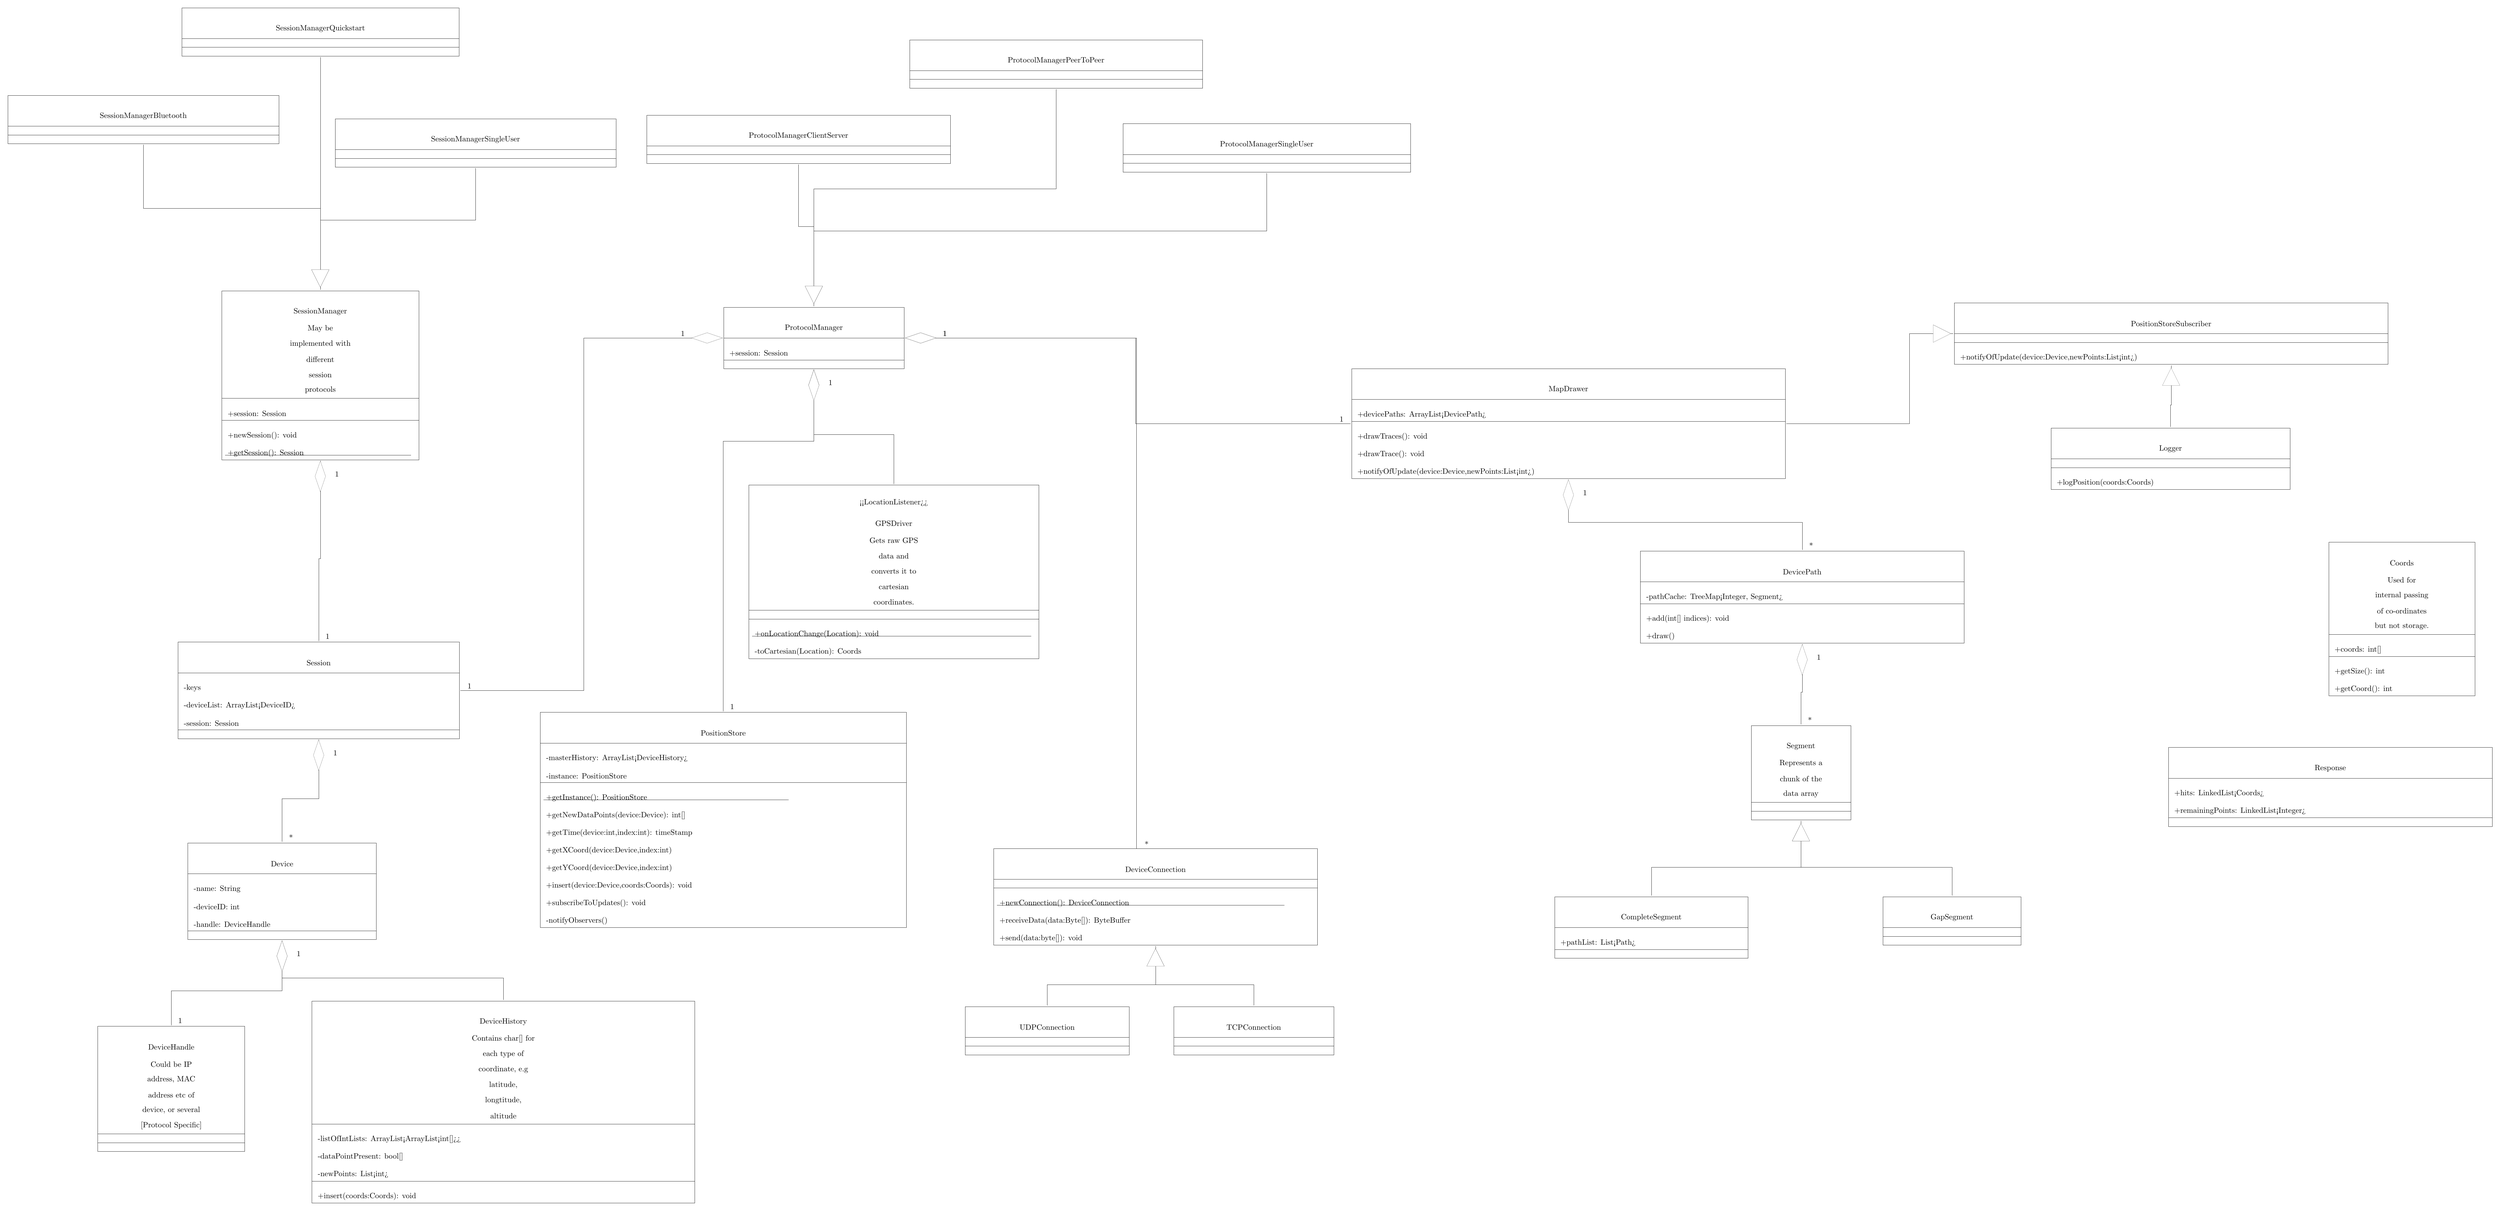
\begin{tikzpicture}
\pgftransformxscale{1.000000}
\pgftransformyscale{-1.000000}
\definecolor{dialinecolor}{rgb}{0.000000, 0.000000, 0.000000}
\pgfsetstrokecolor{dialinecolor}
\definecolor{dialinecolor}{rgb}{1.000000, 1.000000, 1.000000}
\pgfsetfillcolor{dialinecolor}
\pgfsetlinewidth{0.100000\du}
\pgfsetdash{}{0pt}
\definecolor{dialinecolor}{rgb}{1.000000, 1.000000, 1.000000}
\pgfsetfillcolor{dialinecolor}
\fill (-19.700000\du,17.600000\du)--(-19.700000\du,19.000000\du)--(-6.880000\du,19.000000\du)--(-6.880000\du,17.600000\du)--cycle;
\definecolor{dialinecolor}{rgb}{0.000000, 0.000000, 0.000000}
\pgfsetstrokecolor{dialinecolor}
\draw (-19.700000\du,17.600000\du)--(-19.700000\du,19.000000\du)--(-6.880000\du,19.000000\du)--(-6.880000\du,17.600000\du)--cycle;
% setfont left to latex
\definecolor{dialinecolor}{rgb}{0.000000, 0.000000, 0.000000}
\pgfsetstrokecolor{dialinecolor}
\node at (-13.290000\du,18.550000\du){Session};
\definecolor{dialinecolor}{rgb}{1.000000, 1.000000, 1.000000}
\pgfsetfillcolor{dialinecolor}
\fill (-19.700000\du,19.000000\du)--(-19.700000\du,21.600000\du)--(-6.880000\du,21.600000\du)--(-6.880000\du,19.000000\du)--cycle;
\definecolor{dialinecolor}{rgb}{0.000000, 0.000000, 0.000000}
\pgfsetstrokecolor{dialinecolor}
\draw (-19.700000\du,19.000000\du)--(-19.700000\du,21.600000\du)--(-6.880000\du,21.600000\du)--(-6.880000\du,19.000000\du)--cycle;
% setfont left to latex
\definecolor{dialinecolor}{rgb}{0.000000, 0.000000, 0.000000}
\pgfsetstrokecolor{dialinecolor}
\node[anchor=west] at (-19.550000\du,19.700000\du){-keys};
% setfont left to latex
\definecolor{dialinecolor}{rgb}{0.000000, 0.000000, 0.000000}
\pgfsetstrokecolor{dialinecolor}
\node[anchor=west] at (-19.550000\du,20.500000\du){-deviceList: ArrayList<DeviceID>};
% setfont left to latex
\definecolor{dialinecolor}{rgb}{0.000000, 0.000000, 0.000000}
\pgfsetstrokecolor{dialinecolor}
\node[anchor=west] at (-19.550000\du,21.300000\du){-session: Session};
\definecolor{dialinecolor}{rgb}{1.000000, 1.000000, 1.000000}
\pgfsetfillcolor{dialinecolor}
\fill (-19.700000\du,21.600000\du)--(-19.700000\du,22.000000\du)--(-6.880000\du,22.000000\du)--(-6.880000\du,21.600000\du)--cycle;
\definecolor{dialinecolor}{rgb}{0.000000, 0.000000, 0.000000}
\pgfsetstrokecolor{dialinecolor}
\draw (-19.700000\du,21.600000\du)--(-19.700000\du,22.000000\du)--(-6.880000\du,22.000000\du)--(-6.880000\du,21.600000\du)--cycle;
\pgfsetlinewidth{0.100000\du}
\pgfsetdash{}{0pt}
\definecolor{dialinecolor}{rgb}{1.000000, 1.000000, 1.000000}
\pgfsetfillcolor{dialinecolor}
\fill (-19.250000\du,26.750000\du)--(-19.250000\du,28.150000\du)--(-10.665000\du,28.150000\du)--(-10.665000\du,26.750000\du)--cycle;
\definecolor{dialinecolor}{rgb}{0.000000, 0.000000, 0.000000}
\pgfsetstrokecolor{dialinecolor}
\draw (-19.250000\du,26.750000\du)--(-19.250000\du,28.150000\du)--(-10.665000\du,28.150000\du)--(-10.665000\du,26.750000\du)--cycle;
% setfont left to latex
\definecolor{dialinecolor}{rgb}{0.000000, 0.000000, 0.000000}
\pgfsetstrokecolor{dialinecolor}
\node at (-14.957500\du,27.700000\du){Device};
\definecolor{dialinecolor}{rgb}{1.000000, 1.000000, 1.000000}
\pgfsetfillcolor{dialinecolor}
\fill (-19.250000\du,28.150000\du)--(-19.250000\du,30.750000\du)--(-10.665000\du,30.750000\du)--(-10.665000\du,28.150000\du)--cycle;
\definecolor{dialinecolor}{rgb}{0.000000, 0.000000, 0.000000}
\pgfsetstrokecolor{dialinecolor}
\draw (-19.250000\du,28.150000\du)--(-19.250000\du,30.750000\du)--(-10.665000\du,30.750000\du)--(-10.665000\du,28.150000\du)--cycle;
% setfont left to latex
\definecolor{dialinecolor}{rgb}{0.000000, 0.000000, 0.000000}
\pgfsetstrokecolor{dialinecolor}
\node[anchor=west] at (-19.100000\du,28.850000\du){-name: String};
% setfont left to latex
\definecolor{dialinecolor}{rgb}{0.000000, 0.000000, 0.000000}
\pgfsetstrokecolor{dialinecolor}
\node[anchor=west] at (-19.100000\du,29.650000\du){-deviceID: int};
% setfont left to latex
\definecolor{dialinecolor}{rgb}{0.000000, 0.000000, 0.000000}
\pgfsetstrokecolor{dialinecolor}
\node[anchor=west] at (-19.100000\du,30.450000\du){-handle: DeviceHandle};
\definecolor{dialinecolor}{rgb}{1.000000, 1.000000, 1.000000}
\pgfsetfillcolor{dialinecolor}
\fill (-19.250000\du,30.750000\du)--(-19.250000\du,31.150000\du)--(-10.665000\du,31.150000\du)--(-10.665000\du,30.750000\du)--cycle;
\definecolor{dialinecolor}{rgb}{0.000000, 0.000000, 0.000000}
\pgfsetstrokecolor{dialinecolor}
\draw (-19.250000\du,30.750000\du)--(-19.250000\du,31.150000\du)--(-10.665000\du,31.150000\du)--(-10.665000\du,30.750000\du)--cycle;
\pgfsetlinewidth{0.100000\du}
\pgfsetdash{}{0pt}
\definecolor{dialinecolor}{rgb}{1.000000, 1.000000, 1.000000}
\pgfsetfillcolor{dialinecolor}
\fill (-23.350000\du,35.100000\du)--(-23.350000\du,40.000000\du)--(-16.657500\du,40.000000\du)--(-16.657500\du,35.100000\du)--cycle;
\definecolor{dialinecolor}{rgb}{0.000000, 0.000000, 0.000000}
\pgfsetstrokecolor{dialinecolor}
\draw (-23.350000\du,35.100000\du)--(-23.350000\du,40.000000\du)--(-16.657500\du,40.000000\du)--(-16.657500\du,35.100000\du)--cycle;
% setfont left to latex
\definecolor{dialinecolor}{rgb}{0.000000, 0.000000, 0.000000}
\pgfsetstrokecolor{dialinecolor}
\node at (-20.003750\du,36.050000\du){DeviceHandle};
% setfont left to latex
\definecolor{dialinecolor}{rgb}{0.000000, 0.000000, 0.000000}
\pgfsetstrokecolor{dialinecolor}
\node at (-20.003750\du,36.825000\du){Could be IP};
\definecolor{dialinecolor}{rgb}{0.000000, 0.000000, 0.000000}
\pgfsetstrokecolor{dialinecolor}
\node at (-20.003750\du,37.525000\du){address, MAC};
\definecolor{dialinecolor}{rgb}{0.000000, 0.000000, 0.000000}
\pgfsetstrokecolor{dialinecolor}
\node at (-20.003750\du,38.225000\du){address etc of};
\definecolor{dialinecolor}{rgb}{0.000000, 0.000000, 0.000000}
\pgfsetstrokecolor{dialinecolor}
\node at (-20.003750\du,38.925000\du){device, or several};
\definecolor{dialinecolor}{rgb}{0.000000, 0.000000, 0.000000}
\pgfsetstrokecolor{dialinecolor}
\node at (-20.003750\du,39.625000\du){\ensuremath{[}Protocol Specific\ensuremath{]}};
\definecolor{dialinecolor}{rgb}{1.000000, 1.000000, 1.000000}
\pgfsetfillcolor{dialinecolor}
\fill (-23.350000\du,40.000000\du)--(-23.350000\du,40.400000\du)--(-16.657500\du,40.400000\du)--(-16.657500\du,40.000000\du)--cycle;
\definecolor{dialinecolor}{rgb}{0.000000, 0.000000, 0.000000}
\pgfsetstrokecolor{dialinecolor}
\draw (-23.350000\du,40.000000\du)--(-23.350000\du,40.400000\du)--(-16.657500\du,40.400000\du)--(-16.657500\du,40.000000\du)--cycle;
\definecolor{dialinecolor}{rgb}{1.000000, 1.000000, 1.000000}
\pgfsetfillcolor{dialinecolor}
\fill (-23.350000\du,40.400000\du)--(-23.350000\du,40.800000\du)--(-16.657500\du,40.800000\du)--(-16.657500\du,40.400000\du)--cycle;
\definecolor{dialinecolor}{rgb}{0.000000, 0.000000, 0.000000}
\pgfsetstrokecolor{dialinecolor}
\draw (-23.350000\du,40.400000\du)--(-23.350000\du,40.800000\du)--(-16.657500\du,40.800000\du)--(-16.657500\du,40.400000\du)--cycle;
\pgfsetlinewidth{0.100000\du}
\pgfsetdash{}{0pt}
\pgfsetmiterjoin
\pgfsetbuttcap
{
\definecolor{dialinecolor}{rgb}{0.000000, 0.000000, 0.000000}
\pgfsetfillcolor{dialinecolor}
% was here!!!
\definecolor{dialinecolor}{rgb}{0.000000, 0.000000, 0.000000}
\pgfsetstrokecolor{dialinecolor}
\draw (-13.290000\du,22.050275\du)--(-13.290000\du,24.725000\du)--(-14.957500\du,24.725000\du)--(-14.957500\du,26.699725\du);
}
\definecolor{dialinecolor}{rgb}{0.000000, 0.000000, 0.000000}
\pgfsetstrokecolor{dialinecolor}
\draw (-13.290000\du,23.308853\du)--(-13.290000\du,24.725000\du)--(-14.957500\du,24.725000\du)--(-14.957500\du,26.699725\du);
\pgfsetdash{}{0pt}
\pgfsetmiterjoin
\pgfsetbuttcap
\definecolor{dialinecolor}{rgb}{1.000000, 1.000000, 1.000000}
\pgfsetfillcolor{dialinecolor}
\fill (-13.290000\du,22.050275\du)--(-13.050000\du,22.750275\du)--(-13.290000\du,23.450275\du)--(-13.530000\du,22.750275\du)--cycle;
\pgfsetlinewidth{0.100000\du}
\pgfsetdash{}{0pt}
\pgfsetmiterjoin
\pgfsetbuttcap
\definecolor{dialinecolor}{rgb}{0.000000, 0.000000, 0.000000}
\pgfsetstrokecolor{dialinecolor}
\draw (-13.290000\du,22.050275\du)--(-13.050000\du,22.750275\du)--(-13.290000\du,23.450275\du)--(-13.530000\du,22.750275\du)--cycle;
% setfont left to latex
\definecolor{dialinecolor}{rgb}{0.000000, 0.000000, 0.000000}
\pgfsetstrokecolor{dialinecolor}
\node at (-14.123750\du,24.525000\du){};
\definecolor{dialinecolor}{rgb}{0.000000, 0.000000, 0.000000}
\pgfsetstrokecolor{dialinecolor}
\node[anchor=west] at (-12.740000\du,22.650275\du){1};
\definecolor{dialinecolor}{rgb}{0.000000, 0.000000, 0.000000}
\pgfsetstrokecolor{dialinecolor}
\node[anchor=west] at (-14.757500\du,26.499725\du){*};
\pgfsetlinewidth{0.100000\du}
\pgfsetdash{}{0pt}
\pgfsetmiterjoin
\pgfsetbuttcap
{
\definecolor{dialinecolor}{rgb}{0.000000, 0.000000, 0.000000}
\pgfsetfillcolor{dialinecolor}
% was here!!!
\definecolor{dialinecolor}{rgb}{0.000000, 0.000000, 0.000000}
\pgfsetstrokecolor{dialinecolor}
\draw (-14.957500\du,31.200275\du)--(-14.957500\du,33.474960\du)--(-20.003750\du,33.474960\du)--(-20.003750\du,35.049646\du);
}
\definecolor{dialinecolor}{rgb}{0.000000, 0.000000, 0.000000}
\pgfsetstrokecolor{dialinecolor}
\draw (-14.957500\du,32.458853\du)--(-14.957500\du,33.474960\du)--(-20.003750\du,33.474960\du)--(-20.003750\du,35.049646\du);
\pgfsetdash{}{0pt}
\pgfsetmiterjoin
\pgfsetbuttcap
\definecolor{dialinecolor}{rgb}{1.000000, 1.000000, 1.000000}
\pgfsetfillcolor{dialinecolor}
\fill (-14.957500\du,31.200275\du)--(-14.717500\du,31.900275\du)--(-14.957500\du,32.600275\du)--(-15.197500\du,31.900275\du)--cycle;
\pgfsetlinewidth{0.100000\du}
\pgfsetdash{}{0pt}
\pgfsetmiterjoin
\pgfsetbuttcap
\definecolor{dialinecolor}{rgb}{0.000000, 0.000000, 0.000000}
\pgfsetstrokecolor{dialinecolor}
\draw (-14.957500\du,31.200275\du)--(-14.717500\du,31.900275\du)--(-14.957500\du,32.600275\du)--(-15.197500\du,31.900275\du)--cycle;
% setfont left to latex
\definecolor{dialinecolor}{rgb}{0.000000, 0.000000, 0.000000}
\pgfsetstrokecolor{dialinecolor}
\node at (-17.480625\du,33.274960\du){};
\definecolor{dialinecolor}{rgb}{0.000000, 0.000000, 0.000000}
\pgfsetstrokecolor{dialinecolor}
\node[anchor=west] at (-14.407500\du,31.800275\du){1};
\definecolor{dialinecolor}{rgb}{0.000000, 0.000000, 0.000000}
\pgfsetstrokecolor{dialinecolor}
\node[anchor=west] at (-19.803750\du,34.849646\du){1};
\pgfsetlinewidth{0.100000\du}
\pgfsetdash{}{0pt}
\definecolor{dialinecolor}{rgb}{1.000000, 1.000000, 1.000000}
\pgfsetfillcolor{dialinecolor}
\fill (-3.200000\du,20.800000\du)--(-3.200000\du,22.200000\du)--(13.470000\du,22.200000\du)--(13.470000\du,20.800000\du)--cycle;
\definecolor{dialinecolor}{rgb}{0.000000, 0.000000, 0.000000}
\pgfsetstrokecolor{dialinecolor}
\draw (-3.200000\du,20.800000\du)--(-3.200000\du,22.200000\du)--(13.470000\du,22.200000\du)--(13.470000\du,20.800000\du)--cycle;
% setfont left to latex
\definecolor{dialinecolor}{rgb}{0.000000, 0.000000, 0.000000}
\pgfsetstrokecolor{dialinecolor}
\node at (5.135000\du,21.750000\du){PositionStore};
\definecolor{dialinecolor}{rgb}{1.000000, 1.000000, 1.000000}
\pgfsetfillcolor{dialinecolor}
\fill (-3.200000\du,22.200000\du)--(-3.200000\du,24.000000\du)--(13.470000\du,24.000000\du)--(13.470000\du,22.200000\du)--cycle;
\definecolor{dialinecolor}{rgb}{0.000000, 0.000000, 0.000000}
\pgfsetstrokecolor{dialinecolor}
\draw (-3.200000\du,22.200000\du)--(-3.200000\du,24.000000\du)--(13.470000\du,24.000000\du)--(13.470000\du,22.200000\du)--cycle;
% setfont left to latex
\definecolor{dialinecolor}{rgb}{0.000000, 0.000000, 0.000000}
\pgfsetstrokecolor{dialinecolor}
\node[anchor=west] at (-3.050000\du,22.900000\du){-masterHistory: ArrayList<DeviceHistory>};
% setfont left to latex
\definecolor{dialinecolor}{rgb}{0.000000, 0.000000, 0.000000}
\pgfsetstrokecolor{dialinecolor}
\node[anchor=west] at (-3.050000\du,23.700000\du){-instance: PositionStore};
\definecolor{dialinecolor}{rgb}{1.000000, 1.000000, 1.000000}
\pgfsetfillcolor{dialinecolor}
\fill (-3.200000\du,24.000000\du)--(-3.200000\du,30.600000\du)--(13.470000\du,30.600000\du)--(13.470000\du,24.000000\du)--cycle;
\definecolor{dialinecolor}{rgb}{0.000000, 0.000000, 0.000000}
\pgfsetstrokecolor{dialinecolor}
\draw (-3.200000\du,24.000000\du)--(-3.200000\du,30.600000\du)--(13.470000\du,30.600000\du)--(13.470000\du,24.000000\du)--cycle;
% setfont left to latex
\definecolor{dialinecolor}{rgb}{0.000000, 0.000000, 0.000000}
\pgfsetstrokecolor{dialinecolor}
\node[anchor=west] at (-3.050000\du,24.700000\du){+getInstance(): PositionStore};
\pgfsetlinewidth{0.050000\du}
\definecolor{dialinecolor}{rgb}{0.000000, 0.000000, 0.000000}
\pgfsetstrokecolor{dialinecolor}
\draw (-3.050000\du,24.780000\du)--(8.115000\du,24.780000\du);
\pgfsetlinewidth{0.100000\du}
% setfont left to latex
\definecolor{dialinecolor}{rgb}{0.000000, 0.000000, 0.000000}
\pgfsetstrokecolor{dialinecolor}
\node[anchor=west] at (-3.050000\du,25.500000\du){+getNewDataPoints(device:Device): int\ensuremath{[}\ensuremath{]}};
% setfont left to latex
\definecolor{dialinecolor}{rgb}{0.000000, 0.000000, 0.000000}
\pgfsetstrokecolor{dialinecolor}
\node[anchor=west] at (-3.050000\du,26.300000\du){+getTime(device:int,index:int): timeStamp};
% setfont left to latex
\definecolor{dialinecolor}{rgb}{0.000000, 0.000000, 0.000000}
\pgfsetstrokecolor{dialinecolor}
\node[anchor=west] at (-3.050000\du,27.100000\du){+getXCoord(device:Device,index:int)};
% setfont left to latex
\definecolor{dialinecolor}{rgb}{0.000000, 0.000000, 0.000000}
\pgfsetstrokecolor{dialinecolor}
\node[anchor=west] at (-3.050000\du,27.900000\du){+getYCoord(device:Device,index:int)};
% setfont left to latex
\definecolor{dialinecolor}{rgb}{0.000000, 0.000000, 0.000000}
\pgfsetstrokecolor{dialinecolor}
\node[anchor=west] at (-3.050000\du,28.700000\du){+insert(device:Device,coords:Coords): void};
% setfont left to latex
\definecolor{dialinecolor}{rgb}{0.000000, 0.000000, 0.000000}
\pgfsetstrokecolor{dialinecolor}
\node[anchor=west] at (-3.050000\du,29.500000\du){+subscribeToUpdates(): void};
% setfont left to latex
\definecolor{dialinecolor}{rgb}{0.000000, 0.000000, 0.000000}
\pgfsetstrokecolor{dialinecolor}
\node[anchor=west] at (-3.050000\du,30.300000\du){-notifyObservers()};
\pgfsetlinewidth{0.100000\du}
\pgfsetdash{}{0pt}
\definecolor{dialinecolor}{rgb}{1.000000, 1.000000, 1.000000}
\pgfsetfillcolor{dialinecolor}
\fill (-13.600000\du,33.950000\du)--(-13.600000\du,39.550000\du)--(3.840000\du,39.550000\du)--(3.840000\du,33.950000\du)--cycle;
\definecolor{dialinecolor}{rgb}{0.000000, 0.000000, 0.000000}
\pgfsetstrokecolor{dialinecolor}
\draw (-13.600000\du,33.950000\du)--(-13.600000\du,39.550000\du)--(3.840000\du,39.550000\du)--(3.840000\du,33.950000\du)--cycle;
% setfont left to latex
\definecolor{dialinecolor}{rgb}{0.000000, 0.000000, 0.000000}
\pgfsetstrokecolor{dialinecolor}
\node at (-4.880000\du,34.900000\du){DeviceHistory};
% setfont left to latex
\definecolor{dialinecolor}{rgb}{0.000000, 0.000000, 0.000000}
\pgfsetstrokecolor{dialinecolor}
\node at (-4.880000\du,35.675000\du){Contains char\ensuremath{[}\ensuremath{]} for};
\definecolor{dialinecolor}{rgb}{0.000000, 0.000000, 0.000000}
\pgfsetstrokecolor{dialinecolor}
\node at (-4.880000\du,36.375000\du){each type of};
\definecolor{dialinecolor}{rgb}{0.000000, 0.000000, 0.000000}
\pgfsetstrokecolor{dialinecolor}
\node at (-4.880000\du,37.075000\du){coordinate, e.g};
\definecolor{dialinecolor}{rgb}{0.000000, 0.000000, 0.000000}
\pgfsetstrokecolor{dialinecolor}
\node at (-4.880000\du,37.775000\du){latitude,};
\definecolor{dialinecolor}{rgb}{0.000000, 0.000000, 0.000000}
\pgfsetstrokecolor{dialinecolor}
\node at (-4.880000\du,38.475000\du){longtitude,};
\definecolor{dialinecolor}{rgb}{0.000000, 0.000000, 0.000000}
\pgfsetstrokecolor{dialinecolor}
\node at (-4.880000\du,39.175000\du){altitude};
\definecolor{dialinecolor}{rgb}{1.000000, 1.000000, 1.000000}
\pgfsetfillcolor{dialinecolor}
\fill (-13.600000\du,39.550000\du)--(-13.600000\du,42.150000\du)--(3.840000\du,42.150000\du)--(3.840000\du,39.550000\du)--cycle;
\definecolor{dialinecolor}{rgb}{0.000000, 0.000000, 0.000000}
\pgfsetstrokecolor{dialinecolor}
\draw (-13.600000\du,39.550000\du)--(-13.600000\du,42.150000\du)--(3.840000\du,42.150000\du)--(3.840000\du,39.550000\du)--cycle;
% setfont left to latex
\definecolor{dialinecolor}{rgb}{0.000000, 0.000000, 0.000000}
\pgfsetstrokecolor{dialinecolor}
\node[anchor=west] at (-13.450000\du,40.250000\du){-listOfIntLists: ArrayList<ArrayList<int\ensuremath{[}\ensuremath{]}>>};
% setfont left to latex
\definecolor{dialinecolor}{rgb}{0.000000, 0.000000, 0.000000}
\pgfsetstrokecolor{dialinecolor}
\node[anchor=west] at (-13.450000\du,41.050000\du){-dataPointPresent: bool\ensuremath{[}\ensuremath{]}};
% setfont left to latex
\definecolor{dialinecolor}{rgb}{0.000000, 0.000000, 0.000000}
\pgfsetstrokecolor{dialinecolor}
\node[anchor=west] at (-13.450000\du,41.850000\du){-newPoints: List<int>};
\definecolor{dialinecolor}{rgb}{1.000000, 1.000000, 1.000000}
\pgfsetfillcolor{dialinecolor}
\fill (-13.600000\du,42.150000\du)--(-13.600000\du,43.150000\du)--(3.840000\du,43.150000\du)--(3.840000\du,42.150000\du)--cycle;
\definecolor{dialinecolor}{rgb}{0.000000, 0.000000, 0.000000}
\pgfsetstrokecolor{dialinecolor}
\draw (-13.600000\du,42.150000\du)--(-13.600000\du,43.150000\du)--(3.840000\du,43.150000\du)--(3.840000\du,42.150000\du)--cycle;
% setfont left to latex
\definecolor{dialinecolor}{rgb}{0.000000, 0.000000, 0.000000}
\pgfsetstrokecolor{dialinecolor}
\node[anchor=west] at (-13.450000\du,42.850000\du){+insert(coords:Coords): void};
\pgfsetlinewidth{0.100000\du}
\pgfsetdash{}{0pt}
\definecolor{dialinecolor}{rgb}{1.000000, 1.000000, 1.000000}
\pgfsetfillcolor{dialinecolor}
\fill (33.750000\du,5.150000\du)--(33.750000\du,6.550000\du)--(53.500000\du,6.550000\du)--(53.500000\du,5.150000\du)--cycle;
\definecolor{dialinecolor}{rgb}{0.000000, 0.000000, 0.000000}
\pgfsetstrokecolor{dialinecolor}
\draw (33.750000\du,5.150000\du)--(33.750000\du,6.550000\du)--(53.500000\du,6.550000\du)--(53.500000\du,5.150000\du)--cycle;
% setfont left to latex
\definecolor{dialinecolor}{rgb}{0.000000, 0.000000, 0.000000}
\pgfsetstrokecolor{dialinecolor}
\node at (43.625000\du,6.100000\du){MapDrawer};
\definecolor{dialinecolor}{rgb}{1.000000, 1.000000, 1.000000}
\pgfsetfillcolor{dialinecolor}
\fill (33.750000\du,6.550000\du)--(33.750000\du,7.550000\du)--(53.500000\du,7.550000\du)--(53.500000\du,6.550000\du)--cycle;
\definecolor{dialinecolor}{rgb}{0.000000, 0.000000, 0.000000}
\pgfsetstrokecolor{dialinecolor}
\draw (33.750000\du,6.550000\du)--(33.750000\du,7.550000\du)--(53.500000\du,7.550000\du)--(53.500000\du,6.550000\du)--cycle;
% setfont left to latex
\definecolor{dialinecolor}{rgb}{0.000000, 0.000000, 0.000000}
\pgfsetstrokecolor{dialinecolor}
\node[anchor=west] at (33.900000\du,7.250000\du){+devicePaths: ArrayList<DevicePath>};
\definecolor{dialinecolor}{rgb}{1.000000, 1.000000, 1.000000}
\pgfsetfillcolor{dialinecolor}
\fill (33.750000\du,7.550000\du)--(33.750000\du,10.150000\du)--(53.500000\du,10.150000\du)--(53.500000\du,7.550000\du)--cycle;
\definecolor{dialinecolor}{rgb}{0.000000, 0.000000, 0.000000}
\pgfsetstrokecolor{dialinecolor}
\draw (33.750000\du,7.550000\du)--(33.750000\du,10.150000\du)--(53.500000\du,10.150000\du)--(53.500000\du,7.550000\du)--cycle;
% setfont left to latex
\definecolor{dialinecolor}{rgb}{0.000000, 0.000000, 0.000000}
\pgfsetstrokecolor{dialinecolor}
\node[anchor=west] at (33.900000\du,8.250000\du){+drawTraces(): void};
% setfont left to latex
\definecolor{dialinecolor}{rgb}{0.000000, 0.000000, 0.000000}
\pgfsetstrokecolor{dialinecolor}
\node[anchor=west] at (33.900000\du,9.050000\du){+drawTrace(): void};
% setfont left to latex
\definecolor{dialinecolor}{rgb}{0.000000, 0.000000, 0.000000}
\pgfsetstrokecolor{dialinecolor}
\node[anchor=west] at (33.900000\du,9.850000\du){+notifyOfUpdate(device:Device,newPoints:List<int>)};
\pgfsetlinewidth{0.100000\du}
\pgfsetdash{}{0pt}
\definecolor{dialinecolor}{rgb}{1.000000, 1.000000, 1.000000}
\pgfsetfillcolor{dialinecolor}
\fill (46.900000\du,13.450000\du)--(46.900000\du,14.850000\du)--(61.645000\du,14.850000\du)--(61.645000\du,13.450000\du)--cycle;
\definecolor{dialinecolor}{rgb}{0.000000, 0.000000, 0.000000}
\pgfsetstrokecolor{dialinecolor}
\draw (46.900000\du,13.450000\du)--(46.900000\du,14.850000\du)--(61.645000\du,14.850000\du)--(61.645000\du,13.450000\du)--cycle;
% setfont left to latex
\definecolor{dialinecolor}{rgb}{0.000000, 0.000000, 0.000000}
\pgfsetstrokecolor{dialinecolor}
\node at (54.272500\du,14.400000\du){DevicePath};
\definecolor{dialinecolor}{rgb}{1.000000, 1.000000, 1.000000}
\pgfsetfillcolor{dialinecolor}
\fill (46.900000\du,14.850000\du)--(46.900000\du,15.850000\du)--(61.645000\du,15.850000\du)--(61.645000\du,14.850000\du)--cycle;
\definecolor{dialinecolor}{rgb}{0.000000, 0.000000, 0.000000}
\pgfsetstrokecolor{dialinecolor}
\draw (46.900000\du,14.850000\du)--(46.900000\du,15.850000\du)--(61.645000\du,15.850000\du)--(61.645000\du,14.850000\du)--cycle;
% setfont left to latex
\definecolor{dialinecolor}{rgb}{0.000000, 0.000000, 0.000000}
\pgfsetstrokecolor{dialinecolor}
\node[anchor=west] at (47.050000\du,15.550000\du){-pathCache: TreeMap<Integer, Segment>};
\definecolor{dialinecolor}{rgb}{1.000000, 1.000000, 1.000000}
\pgfsetfillcolor{dialinecolor}
\fill (46.900000\du,15.850000\du)--(46.900000\du,17.650000\du)--(61.645000\du,17.650000\du)--(61.645000\du,15.850000\du)--cycle;
\definecolor{dialinecolor}{rgb}{0.000000, 0.000000, 0.000000}
\pgfsetstrokecolor{dialinecolor}
\draw (46.900000\du,15.850000\du)--(46.900000\du,17.650000\du)--(61.645000\du,17.650000\du)--(61.645000\du,15.850000\du)--cycle;
% setfont left to latex
\definecolor{dialinecolor}{rgb}{0.000000, 0.000000, 0.000000}
\pgfsetstrokecolor{dialinecolor}
\node[anchor=west] at (47.050000\du,16.550000\du){+add(int\ensuremath{[}\ensuremath{]} indices): void};
% setfont left to latex
\definecolor{dialinecolor}{rgb}{0.000000, 0.000000, 0.000000}
\pgfsetstrokecolor{dialinecolor}
\node[anchor=west] at (47.050000\du,17.350000\du){+draw()};
\pgfsetlinewidth{0.100000\du}
\pgfsetdash{}{0pt}
\pgfsetmiterjoin
\pgfsetbuttcap
{
\definecolor{dialinecolor}{rgb}{0.000000, 0.000000, 0.000000}
\pgfsetfillcolor{dialinecolor}
% was here!!!
\definecolor{dialinecolor}{rgb}{0.000000, 0.000000, 0.000000}
\pgfsetstrokecolor{dialinecolor}
\draw (43.625000\du,10.200311\du)--(43.625000\du,12.150024\du)--(54.272500\du,12.150024\du)--(54.272500\du,13.399738\du);
}
\definecolor{dialinecolor}{rgb}{0.000000, 0.000000, 0.000000}
\pgfsetstrokecolor{dialinecolor}
\draw (43.625000\du,11.458890\du)--(43.625000\du,12.150024\du)--(54.272500\du,12.150024\du)--(54.272500\du,13.399738\du);
\pgfsetdash{}{0pt}
\pgfsetmiterjoin
\pgfsetbuttcap
\definecolor{dialinecolor}{rgb}{1.000000, 1.000000, 1.000000}
\pgfsetfillcolor{dialinecolor}
\fill (43.625000\du,10.200311\du)--(43.865000\du,10.900311\du)--(43.625000\du,11.600311\du)--(43.385000\du,10.900311\du)--cycle;
\pgfsetlinewidth{0.100000\du}
\pgfsetdash{}{0pt}
\pgfsetmiterjoin
\pgfsetbuttcap
\definecolor{dialinecolor}{rgb}{0.000000, 0.000000, 0.000000}
\pgfsetstrokecolor{dialinecolor}
\draw (43.625000\du,10.200311\du)--(43.865000\du,10.900311\du)--(43.625000\du,11.600311\du)--(43.385000\du,10.900311\du)--cycle;
% setfont left to latex
\definecolor{dialinecolor}{rgb}{0.000000, 0.000000, 0.000000}
\pgfsetstrokecolor{dialinecolor}
\node at (48.948750\du,11.950024\du){};
\definecolor{dialinecolor}{rgb}{0.000000, 0.000000, 0.000000}
\pgfsetstrokecolor{dialinecolor}
\node[anchor=west] at (44.175000\du,10.800311\du){1};
\definecolor{dialinecolor}{rgb}{0.000000, 0.000000, 0.000000}
\pgfsetstrokecolor{dialinecolor}
\node[anchor=west] at (54.472500\du,13.199738\du){*};
\pgfsetlinewidth{0.100000\du}
\pgfsetdash{}{0pt}
\definecolor{dialinecolor}{rgb}{1.000000, 1.000000, 1.000000}
\pgfsetfillcolor{dialinecolor}
\fill (5.150000\du,2.350000\du)--(5.150000\du,3.750000\du)--(13.372500\du,3.750000\du)--(13.372500\du,2.350000\du)--cycle;
\definecolor{dialinecolor}{rgb}{0.000000, 0.000000, 0.000000}
\pgfsetstrokecolor{dialinecolor}
\draw (5.150000\du,2.350000\du)--(5.150000\du,3.750000\du)--(13.372500\du,3.750000\du)--(13.372500\du,2.350000\du)--cycle;
% setfont left to latex
\definecolor{dialinecolor}{rgb}{0.000000, 0.000000, 0.000000}
\pgfsetstrokecolor{dialinecolor}
\node at (9.261250\du,3.300000\du){ProtocolManager};
\definecolor{dialinecolor}{rgb}{1.000000, 1.000000, 1.000000}
\pgfsetfillcolor{dialinecolor}
\fill (5.150000\du,3.750000\du)--(5.150000\du,4.750000\du)--(13.372500\du,4.750000\du)--(13.372500\du,3.750000\du)--cycle;
\definecolor{dialinecolor}{rgb}{0.000000, 0.000000, 0.000000}
\pgfsetstrokecolor{dialinecolor}
\draw (5.150000\du,3.750000\du)--(5.150000\du,4.750000\du)--(13.372500\du,4.750000\du)--(13.372500\du,3.750000\du)--cycle;
% setfont left to latex
\definecolor{dialinecolor}{rgb}{0.000000, 0.000000, 0.000000}
\pgfsetstrokecolor{dialinecolor}
\node[anchor=west] at (5.300000\du,4.450000\du){+session: Session};
\definecolor{dialinecolor}{rgb}{1.000000, 1.000000, 1.000000}
\pgfsetfillcolor{dialinecolor}
\fill (5.150000\du,4.750000\du)--(5.150000\du,5.150000\du)--(13.372500\du,5.150000\du)--(13.372500\du,4.750000\du)--cycle;
\definecolor{dialinecolor}{rgb}{0.000000, 0.000000, 0.000000}
\pgfsetstrokecolor{dialinecolor}
\draw (5.150000\du,4.750000\du)--(5.150000\du,5.150000\du)--(13.372500\du,5.150000\du)--(13.372500\du,4.750000\du)--cycle;
\pgfsetlinewidth{0.100000\du}
\pgfsetdash{}{0pt}
\pgfsetmiterjoin
\pgfsetbuttcap
{
\definecolor{dialinecolor}{rgb}{0.000000, 0.000000, 0.000000}
\pgfsetfillcolor{dialinecolor}
% was here!!!
\definecolor{dialinecolor}{rgb}{0.000000, 0.000000, 0.000000}
\pgfsetstrokecolor{dialinecolor}
\draw (5.099746\du,3.750000\du)--(-1.214930\du,3.750000\du)--(-1.214930\du,19.800000\du)--(-6.829606\du,19.800000\du);
}
\definecolor{dialinecolor}{rgb}{0.000000, 0.000000, 0.000000}
\pgfsetstrokecolor{dialinecolor}
\draw (3.841167\du,3.750000\du)--(-1.214930\du,3.750000\du)--(-1.214930\du,19.800000\du)--(-6.829606\du,19.800000\du);
\pgfsetdash{}{0pt}
\pgfsetmiterjoin
\pgfsetbuttcap
\definecolor{dialinecolor}{rgb}{1.000000, 1.000000, 1.000000}
\pgfsetfillcolor{dialinecolor}
\fill (5.099746\du,3.750000\du)--(4.399746\du,3.990000\du)--(3.699746\du,3.750000\du)--(4.399746\du,3.510000\du)--cycle;
\pgfsetlinewidth{0.100000\du}
\pgfsetdash{}{0pt}
\pgfsetmiterjoin
\pgfsetbuttcap
\definecolor{dialinecolor}{rgb}{0.000000, 0.000000, 0.000000}
\pgfsetstrokecolor{dialinecolor}
\draw (5.099746\du,3.750000\du)--(4.399746\du,3.990000\du)--(3.699746\du,3.750000\du)--(4.399746\du,3.510000\du)--cycle;
% setfont left to latex
\definecolor{dialinecolor}{rgb}{0.000000, 0.000000, 0.000000}
\pgfsetstrokecolor{dialinecolor}
\node[anchor=west] at (-1.114930\du,11.575000\du){};
\definecolor{dialinecolor}{rgb}{0.000000, 0.000000, 0.000000}
\pgfsetstrokecolor{dialinecolor}
\node[anchor=east] at (3.499746\du,3.550000\du){1};
\definecolor{dialinecolor}{rgb}{0.000000, 0.000000, 0.000000}
\pgfsetstrokecolor{dialinecolor}
\node[anchor=west] at (-6.629606\du,19.600000\du){1};
\pgfsetlinewidth{0.100000\du}
\pgfsetdash{}{0pt}
\pgfsetmiterjoin
\pgfsetbuttcap
{
\definecolor{dialinecolor}{rgb}{0.000000, 0.000000, 0.000000}
\pgfsetfillcolor{dialinecolor}
% was here!!!
\definecolor{dialinecolor}{rgb}{0.000000, 0.000000, 0.000000}
\pgfsetstrokecolor{dialinecolor}
\draw (9.261250\du,5.191211\du)--(9.261250\du,8.450000\du)--(5.135000\du,8.450000\du)--(5.135000\du,20.750522\du);
}
\definecolor{dialinecolor}{rgb}{0.000000, 0.000000, 0.000000}
\pgfsetstrokecolor{dialinecolor}
\draw (9.261250\du,6.449790\du)--(9.261250\du,8.450000\du)--(5.135000\du,8.450000\du)--(5.135000\du,20.750522\du);
\pgfsetdash{}{0pt}
\pgfsetmiterjoin
\pgfsetbuttcap
\definecolor{dialinecolor}{rgb}{1.000000, 1.000000, 1.000000}
\pgfsetfillcolor{dialinecolor}
\fill (9.261250\du,5.191211\du)--(9.501250\du,5.891211\du)--(9.261250\du,6.591211\du)--(9.021250\du,5.891211\du)--cycle;
\pgfsetlinewidth{0.100000\du}
\pgfsetdash{}{0pt}
\pgfsetmiterjoin
\pgfsetbuttcap
\definecolor{dialinecolor}{rgb}{0.000000, 0.000000, 0.000000}
\pgfsetstrokecolor{dialinecolor}
\draw (9.261250\du,5.191211\du)--(9.501250\du,5.891211\du)--(9.261250\du,6.591211\du)--(9.021250\du,5.891211\du)--cycle;
% setfont left to latex
\definecolor{dialinecolor}{rgb}{0.000000, 0.000000, 0.000000}
\pgfsetstrokecolor{dialinecolor}
\node at (7.198125\du,8.250000\du){};
\definecolor{dialinecolor}{rgb}{0.000000, 0.000000, 0.000000}
\pgfsetstrokecolor{dialinecolor}
\node[anchor=west] at (9.811250\du,5.791211\du){1};
\definecolor{dialinecolor}{rgb}{0.000000, 0.000000, 0.000000}
\pgfsetstrokecolor{dialinecolor}
\node[anchor=west] at (5.335000\du,20.550522\du){1};
\pgfsetlinewidth{0.100000\du}
\pgfsetdash{}{0pt}
\pgfsetmiterjoin
\pgfsetbuttcap
{
\definecolor{dialinecolor}{rgb}{0.000000, 0.000000, 0.000000}
\pgfsetfillcolor{dialinecolor}
% was here!!!
\definecolor{dialinecolor}{rgb}{0.000000, 0.000000, 0.000000}
\pgfsetstrokecolor{dialinecolor}
\draw (13.422754\du,3.750000\du)--(23.911226\du,3.750000\du)--(23.911226\du,7.650000\du)--(33.699697\du,7.650000\du);
}
\definecolor{dialinecolor}{rgb}{0.000000, 0.000000, 0.000000}
\pgfsetstrokecolor{dialinecolor}
\draw (14.681333\du,3.750000\du)--(23.911226\du,3.750000\du)--(23.911226\du,7.650000\du)--(33.699697\du,7.650000\du);
\pgfsetdash{}{0pt}
\pgfsetmiterjoin
\pgfsetbuttcap
\definecolor{dialinecolor}{rgb}{1.000000, 1.000000, 1.000000}
\pgfsetfillcolor{dialinecolor}
\fill (13.422754\du,3.750000\du)--(14.122754\du,3.510000\du)--(14.822754\du,3.750000\du)--(14.122754\du,3.990000\du)--cycle;
\pgfsetlinewidth{0.100000\du}
\pgfsetdash{}{0pt}
\pgfsetmiterjoin
\pgfsetbuttcap
\definecolor{dialinecolor}{rgb}{0.000000, 0.000000, 0.000000}
\pgfsetstrokecolor{dialinecolor}
\draw (13.422754\du,3.750000\du)--(14.122754\du,3.510000\du)--(14.822754\du,3.750000\du)--(14.122754\du,3.990000\du)--cycle;
% setfont left to latex
\definecolor{dialinecolor}{rgb}{0.000000, 0.000000, 0.000000}
\pgfsetstrokecolor{dialinecolor}
\node[anchor=west] at (24.011226\du,5.500000\du){};
\definecolor{dialinecolor}{rgb}{0.000000, 0.000000, 0.000000}
\pgfsetstrokecolor{dialinecolor}
\node[anchor=west] at (15.022754\du,3.550000\du){1};
\definecolor{dialinecolor}{rgb}{0.000000, 0.000000, 0.000000}
\pgfsetstrokecolor{dialinecolor}
\node[anchor=east] at (33.499697\du,7.450000\du){1};
\pgfsetlinewidth{0.100000\du}
\pgfsetdash{}{0pt}
\definecolor{dialinecolor}{rgb}{1.000000, 1.000000, 1.000000}
\pgfsetfillcolor{dialinecolor}
\fill (-17.700000\du,1.600000\du)--(-17.700000\du,6.500000\du)--(-8.730000\du,6.500000\du)--(-8.730000\du,1.600000\du)--cycle;
\definecolor{dialinecolor}{rgb}{0.000000, 0.000000, 0.000000}
\pgfsetstrokecolor{dialinecolor}
\draw (-17.700000\du,1.600000\du)--(-17.700000\du,6.500000\du)--(-8.730000\du,6.500000\du)--(-8.730000\du,1.600000\du)--cycle;
% setfont left to latex
\definecolor{dialinecolor}{rgb}{0.000000, 0.000000, 0.000000}
\pgfsetstrokecolor{dialinecolor}
\node at (-13.215000\du,2.550000\du){SessionManager};
% setfont left to latex
\definecolor{dialinecolor}{rgb}{0.000000, 0.000000, 0.000000}
\pgfsetstrokecolor{dialinecolor}
\node at (-13.215000\du,3.325000\du){May be};
\definecolor{dialinecolor}{rgb}{0.000000, 0.000000, 0.000000}
\pgfsetstrokecolor{dialinecolor}
\node at (-13.215000\du,4.025000\du){implemented with};
\definecolor{dialinecolor}{rgb}{0.000000, 0.000000, 0.000000}
\pgfsetstrokecolor{dialinecolor}
\node at (-13.215000\du,4.725000\du){different};
\definecolor{dialinecolor}{rgb}{0.000000, 0.000000, 0.000000}
\pgfsetstrokecolor{dialinecolor}
\node at (-13.215000\du,5.425000\du){session};
\definecolor{dialinecolor}{rgb}{0.000000, 0.000000, 0.000000}
\pgfsetstrokecolor{dialinecolor}
\node at (-13.215000\du,6.125000\du){protocols};
\definecolor{dialinecolor}{rgb}{1.000000, 1.000000, 1.000000}
\pgfsetfillcolor{dialinecolor}
\fill (-17.700000\du,6.500000\du)--(-17.700000\du,7.500000\du)--(-8.730000\du,7.500000\du)--(-8.730000\du,6.500000\du)--cycle;
\definecolor{dialinecolor}{rgb}{0.000000, 0.000000, 0.000000}
\pgfsetstrokecolor{dialinecolor}
\draw (-17.700000\du,6.500000\du)--(-17.700000\du,7.500000\du)--(-8.730000\du,7.500000\du)--(-8.730000\du,6.500000\du)--cycle;
% setfont left to latex
\definecolor{dialinecolor}{rgb}{0.000000, 0.000000, 0.000000}
\pgfsetstrokecolor{dialinecolor}
\node[anchor=west] at (-17.550000\du,7.200000\du){+session: Session};
\definecolor{dialinecolor}{rgb}{1.000000, 1.000000, 1.000000}
\pgfsetfillcolor{dialinecolor}
\fill (-17.700000\du,7.500000\du)--(-17.700000\du,9.300000\du)--(-8.730000\du,9.300000\du)--(-8.730000\du,7.500000\du)--cycle;
\definecolor{dialinecolor}{rgb}{0.000000, 0.000000, 0.000000}
\pgfsetstrokecolor{dialinecolor}
\draw (-17.700000\du,7.500000\du)--(-17.700000\du,9.300000\du)--(-8.730000\du,9.300000\du)--(-8.730000\du,7.500000\du)--cycle;
% setfont left to latex
\definecolor{dialinecolor}{rgb}{0.000000, 0.000000, 0.000000}
\pgfsetstrokecolor{dialinecolor}
\node[anchor=west] at (-17.550000\du,8.200000\du){+newSession(): void};
% setfont left to latex
\definecolor{dialinecolor}{rgb}{0.000000, 0.000000, 0.000000}
\pgfsetstrokecolor{dialinecolor}
\node[anchor=west] at (-17.550000\du,9.000000\du){+getSession(): Session};
\pgfsetlinewidth{0.050000\du}
\definecolor{dialinecolor}{rgb}{0.000000, 0.000000, 0.000000}
\pgfsetstrokecolor{dialinecolor}
\draw (-17.550000\du,9.080000\du)--(-9.080000\du,9.080000\du);
\pgfsetlinewidth{0.100000\du}
\pgfsetlinewidth{0.100000\du}
\pgfsetdash{}{0pt}
\pgfsetmiterjoin
\pgfsetbuttcap
{
\definecolor{dialinecolor}{rgb}{0.000000, 0.000000, 0.000000}
\pgfsetfillcolor{dialinecolor}
% was here!!!
\definecolor{dialinecolor}{rgb}{0.000000, 0.000000, 0.000000}
\pgfsetstrokecolor{dialinecolor}
\draw (-13.215000\du,9.350476\du)--(-13.215000\du,13.800101\du)--(-13.290000\du,13.800101\du)--(-13.290000\du,17.549725\du);
}
\definecolor{dialinecolor}{rgb}{0.000000, 0.000000, 0.000000}
\pgfsetstrokecolor{dialinecolor}
\draw (-13.215000\du,10.609055\du)--(-13.215000\du,13.800101\du)--(-13.290000\du,13.800101\du)--(-13.290000\du,17.549725\du);
\pgfsetdash{}{0pt}
\pgfsetmiterjoin
\pgfsetbuttcap
\definecolor{dialinecolor}{rgb}{1.000000, 1.000000, 1.000000}
\pgfsetfillcolor{dialinecolor}
\fill (-13.215000\du,9.350476\du)--(-12.975000\du,10.050476\du)--(-13.215000\du,10.750476\du)--(-13.455000\du,10.050476\du)--cycle;
\pgfsetlinewidth{0.100000\du}
\pgfsetdash{}{0pt}
\pgfsetmiterjoin
\pgfsetbuttcap
\definecolor{dialinecolor}{rgb}{0.000000, 0.000000, 0.000000}
\pgfsetstrokecolor{dialinecolor}
\draw (-13.215000\du,9.350476\du)--(-12.975000\du,10.050476\du)--(-13.215000\du,10.750476\du)--(-13.455000\du,10.050476\du)--cycle;
% setfont left to latex
\definecolor{dialinecolor}{rgb}{0.000000, 0.000000, 0.000000}
\pgfsetstrokecolor{dialinecolor}
\node at (-13.252500\du,13.600101\du){};
\definecolor{dialinecolor}{rgb}{0.000000, 0.000000, 0.000000}
\pgfsetstrokecolor{dialinecolor}
\node[anchor=west] at (-12.665000\du,9.950476\du){1};
\definecolor{dialinecolor}{rgb}{0.000000, 0.000000, 0.000000}
\pgfsetstrokecolor{dialinecolor}
\node[anchor=west] at (-13.090000\du,17.349725\du){1};
\pgfsetlinewidth{0.100000\du}
\pgfsetdash{}{0pt}
\definecolor{dialinecolor}{rgb}{1.000000, 1.000000, 1.000000}
\pgfsetfillcolor{dialinecolor}
\fill (78.250000\du,13.050000\du)--(78.250000\du,17.250000\du)--(84.910000\du,17.250000\du)--(84.910000\du,13.050000\du)--cycle;
\definecolor{dialinecolor}{rgb}{0.000000, 0.000000, 0.000000}
\pgfsetstrokecolor{dialinecolor}
\draw (78.250000\du,13.050000\du)--(78.250000\du,17.250000\du)--(84.910000\du,17.250000\du)--(84.910000\du,13.050000\du)--cycle;
% setfont left to latex
\definecolor{dialinecolor}{rgb}{0.000000, 0.000000, 0.000000}
\pgfsetstrokecolor{dialinecolor}
\node at (81.580000\du,14.000000\du){Coords};
% setfont left to latex
\definecolor{dialinecolor}{rgb}{0.000000, 0.000000, 0.000000}
\pgfsetstrokecolor{dialinecolor}
\node at (81.580000\du,14.775000\du){Used for};
\definecolor{dialinecolor}{rgb}{0.000000, 0.000000, 0.000000}
\pgfsetstrokecolor{dialinecolor}
\node at (81.580000\du,15.475000\du){internal passing};
\definecolor{dialinecolor}{rgb}{0.000000, 0.000000, 0.000000}
\pgfsetstrokecolor{dialinecolor}
\node at (81.580000\du,16.175000\du){of co-ordinates};
\definecolor{dialinecolor}{rgb}{0.000000, 0.000000, 0.000000}
\pgfsetstrokecolor{dialinecolor}
\node at (81.580000\du,16.875000\du){but not storage.};
\definecolor{dialinecolor}{rgb}{1.000000, 1.000000, 1.000000}
\pgfsetfillcolor{dialinecolor}
\fill (78.250000\du,17.250000\du)--(78.250000\du,18.250000\du)--(84.910000\du,18.250000\du)--(84.910000\du,17.250000\du)--cycle;
\definecolor{dialinecolor}{rgb}{0.000000, 0.000000, 0.000000}
\pgfsetstrokecolor{dialinecolor}
\draw (78.250000\du,17.250000\du)--(78.250000\du,18.250000\du)--(84.910000\du,18.250000\du)--(84.910000\du,17.250000\du)--cycle;
% setfont left to latex
\definecolor{dialinecolor}{rgb}{0.000000, 0.000000, 0.000000}
\pgfsetstrokecolor{dialinecolor}
\node[anchor=west] at (78.400000\du,17.950000\du){+coords: int\ensuremath{[}\ensuremath{]}};
\definecolor{dialinecolor}{rgb}{1.000000, 1.000000, 1.000000}
\pgfsetfillcolor{dialinecolor}
\fill (78.250000\du,18.250000\du)--(78.250000\du,20.050000\du)--(84.910000\du,20.050000\du)--(84.910000\du,18.250000\du)--cycle;
\definecolor{dialinecolor}{rgb}{0.000000, 0.000000, 0.000000}
\pgfsetstrokecolor{dialinecolor}
\draw (78.250000\du,18.250000\du)--(78.250000\du,20.050000\du)--(84.910000\du,20.050000\du)--(84.910000\du,18.250000\du)--cycle;
% setfont left to latex
\definecolor{dialinecolor}{rgb}{0.000000, 0.000000, 0.000000}
\pgfsetstrokecolor{dialinecolor}
\node[anchor=west] at (78.400000\du,18.950000\du){+getSize(): int};
% setfont left to latex
\definecolor{dialinecolor}{rgb}{0.000000, 0.000000, 0.000000}
\pgfsetstrokecolor{dialinecolor}
\node[anchor=west] at (78.400000\du,19.750000\du){+getCoord(): int};
\pgfsetlinewidth{0.100000\du}
\pgfsetdash{}{0pt}
\definecolor{dialinecolor}{rgb}{1.000000, 1.000000, 1.000000}
\pgfsetfillcolor{dialinecolor}
\fill (6.300000\du,10.450000\du)--(6.300000\du,16.150000\du)--(19.505000\du,16.150000\du)--(19.505000\du,10.450000\du)--cycle;
\definecolor{dialinecolor}{rgb}{0.000000, 0.000000, 0.000000}
\pgfsetstrokecolor{dialinecolor}
\draw (6.300000\du,10.450000\du)--(6.300000\du,16.150000\du)--(19.505000\du,16.150000\du)--(19.505000\du,10.450000\du)--cycle;
% setfont left to latex
\definecolor{dialinecolor}{rgb}{0.000000, 0.000000, 0.000000}
\pgfsetstrokecolor{dialinecolor}
\node at (12.902500\du,11.250000\du){<<LocationListener>>};
% setfont left to latex
\definecolor{dialinecolor}{rgb}{0.000000, 0.000000, 0.000000}
\pgfsetstrokecolor{dialinecolor}
\node at (12.902500\du,12.200000\du){GPSDriver};
% setfont left to latex
\definecolor{dialinecolor}{rgb}{0.000000, 0.000000, 0.000000}
\pgfsetstrokecolor{dialinecolor}
\node at (12.902500\du,12.975000\du){Gets raw GPS};
\definecolor{dialinecolor}{rgb}{0.000000, 0.000000, 0.000000}
\pgfsetstrokecolor{dialinecolor}
\node at (12.902500\du,13.675000\du){data and};
\definecolor{dialinecolor}{rgb}{0.000000, 0.000000, 0.000000}
\pgfsetstrokecolor{dialinecolor}
\node at (12.902500\du,14.375000\du){converts it to};
\definecolor{dialinecolor}{rgb}{0.000000, 0.000000, 0.000000}
\pgfsetstrokecolor{dialinecolor}
\node at (12.902500\du,15.075000\du){cartesian};
\definecolor{dialinecolor}{rgb}{0.000000, 0.000000, 0.000000}
\pgfsetstrokecolor{dialinecolor}
\node at (12.902500\du,15.775000\du){coordinates.};
\definecolor{dialinecolor}{rgb}{1.000000, 1.000000, 1.000000}
\pgfsetfillcolor{dialinecolor}
\fill (6.300000\du,16.150000\du)--(6.300000\du,16.550000\du)--(19.505000\du,16.550000\du)--(19.505000\du,16.150000\du)--cycle;
\definecolor{dialinecolor}{rgb}{0.000000, 0.000000, 0.000000}
\pgfsetstrokecolor{dialinecolor}
\draw (6.300000\du,16.150000\du)--(6.300000\du,16.550000\du)--(19.505000\du,16.550000\du)--(19.505000\du,16.150000\du)--cycle;
\definecolor{dialinecolor}{rgb}{1.000000, 1.000000, 1.000000}
\pgfsetfillcolor{dialinecolor}
\fill (6.300000\du,16.550000\du)--(6.300000\du,18.350000\du)--(19.505000\du,18.350000\du)--(19.505000\du,16.550000\du)--cycle;
\definecolor{dialinecolor}{rgb}{0.000000, 0.000000, 0.000000}
\pgfsetstrokecolor{dialinecolor}
\draw (6.300000\du,16.550000\du)--(6.300000\du,18.350000\du)--(19.505000\du,18.350000\du)--(19.505000\du,16.550000\du)--cycle;
% setfont left to latex
\definecolor{dialinecolor}{rgb}{0.000000, 0.000000, 0.000000}
\pgfsetstrokecolor{dialinecolor}
\node[anchor=west] at (6.450000\du,17.250000\du){+onLocationChange(Location): void};
\pgfsetlinewidth{0.050000\du}
\definecolor{dialinecolor}{rgb}{0.000000, 0.000000, 0.000000}
\pgfsetstrokecolor{dialinecolor}
\draw (6.450000\du,17.330000\du)--(19.155000\du,17.330000\du);
\pgfsetlinewidth{0.100000\du}
% setfont left to latex
\definecolor{dialinecolor}{rgb}{0.000000, 0.000000, 0.000000}
\pgfsetstrokecolor{dialinecolor}
\node[anchor=west] at (6.450000\du,18.050000\du){-toCartesian(Location): Coords};
\pgfsetlinewidth{0.100000\du}
\pgfsetdash{}{0pt}
\pgfsetmiterjoin
\pgfsetbuttcap
{
\definecolor{dialinecolor}{rgb}{0.000000, 0.000000, 0.000000}
\pgfsetfillcolor{dialinecolor}
% was here!!!
\definecolor{dialinecolor}{rgb}{0.000000, 0.000000, 0.000000}
\pgfsetstrokecolor{dialinecolor}
\draw (9.261250\du,5.200354\du)--(9.261250\du,8.149933\du)--(12.902500\du,8.149933\du)--(12.902500\du,10.399512\du);
}
\definecolor{dialinecolor}{rgb}{0.000000, 0.000000, 0.000000}
\pgfsetstrokecolor{dialinecolor}
\draw (9.261250\du,6.458933\du)--(9.261250\du,8.149933\du)--(12.902500\du,8.149933\du)--(12.902500\du,10.399512\du);
\pgfsetdash{}{0pt}
\pgfsetmiterjoin
\pgfsetbuttcap
\definecolor{dialinecolor}{rgb}{1.000000, 1.000000, 1.000000}
\pgfsetfillcolor{dialinecolor}
\fill (9.261250\du,5.200354\du)--(9.501250\du,5.900354\du)--(9.261250\du,6.600354\du)--(9.021250\du,5.900354\du)--cycle;
\pgfsetlinewidth{0.100000\du}
\pgfsetdash{}{0pt}
\pgfsetmiterjoin
\pgfsetbuttcap
\definecolor{dialinecolor}{rgb}{0.000000, 0.000000, 0.000000}
\pgfsetstrokecolor{dialinecolor}
\draw (9.261250\du,5.200354\du)--(9.501250\du,5.900354\du)--(9.261250\du,6.600354\du)--(9.021250\du,5.900354\du)--cycle;
% setfont left to latex
\definecolor{dialinecolor}{rgb}{0.000000, 0.000000, 0.000000}
\pgfsetstrokecolor{dialinecolor}
\node at (11.081875\du,7.949933\du){};
\definecolor{dialinecolor}{rgb}{0.000000, 0.000000, 0.000000}
\pgfsetstrokecolor{dialinecolor}
\node[anchor=west] at (9.811250\du,5.800354\du){};
\definecolor{dialinecolor}{rgb}{0.000000, 0.000000, 0.000000}
\pgfsetstrokecolor{dialinecolor}
\node[anchor=west] at (13.102500\du,10.199512\du){};
\pgfsetlinewidth{0.100000\du}
\pgfsetdash{}{0pt}
\definecolor{dialinecolor}{rgb}{1.000000, 1.000000, 1.000000}
\pgfsetfillcolor{dialinecolor}
\fill (65.600000\du,7.850000\du)--(65.600000\du,9.250000\du)--(76.495000\du,9.250000\du)--(76.495000\du,7.850000\du)--cycle;
\definecolor{dialinecolor}{rgb}{0.000000, 0.000000, 0.000000}
\pgfsetstrokecolor{dialinecolor}
\draw (65.600000\du,7.850000\du)--(65.600000\du,9.250000\du)--(76.495000\du,9.250000\du)--(76.495000\du,7.850000\du)--cycle;
% setfont left to latex
\definecolor{dialinecolor}{rgb}{0.000000, 0.000000, 0.000000}
\pgfsetstrokecolor{dialinecolor}
\node at (71.047500\du,8.800000\du){Logger};
\definecolor{dialinecolor}{rgb}{1.000000, 1.000000, 1.000000}
\pgfsetfillcolor{dialinecolor}
\fill (65.600000\du,9.250000\du)--(65.600000\du,9.650000\du)--(76.495000\du,9.650000\du)--(76.495000\du,9.250000\du)--cycle;
\definecolor{dialinecolor}{rgb}{0.000000, 0.000000, 0.000000}
\pgfsetstrokecolor{dialinecolor}
\draw (65.600000\du,9.250000\du)--(65.600000\du,9.650000\du)--(76.495000\du,9.650000\du)--(76.495000\du,9.250000\du)--cycle;
\definecolor{dialinecolor}{rgb}{1.000000, 1.000000, 1.000000}
\pgfsetfillcolor{dialinecolor}
\fill (65.600000\du,9.650000\du)--(65.600000\du,10.650000\du)--(76.495000\du,10.650000\du)--(76.495000\du,9.650000\du)--cycle;
\definecolor{dialinecolor}{rgb}{0.000000, 0.000000, 0.000000}
\pgfsetstrokecolor{dialinecolor}
\draw (65.600000\du,9.650000\du)--(65.600000\du,10.650000\du)--(76.495000\du,10.650000\du)--(76.495000\du,9.650000\du)--cycle;
% setfont left to latex
\definecolor{dialinecolor}{rgb}{0.000000, 0.000000, 0.000000}
\pgfsetstrokecolor{dialinecolor}
\node[anchor=west] at (65.750000\du,10.350000\du){+logPosition(coords:Coords)};
\pgfsetlinewidth{0.100000\du}
\pgfsetdash{}{0pt}
\definecolor{dialinecolor}{rgb}{1.000000, 1.000000, 1.000000}
\pgfsetfillcolor{dialinecolor}
\fill (51.950000\du,21.400000\du)--(51.950000\du,24.900000\du)--(56.482500\du,24.900000\du)--(56.482500\du,21.400000\du)--cycle;
\definecolor{dialinecolor}{rgb}{0.000000, 0.000000, 0.000000}
\pgfsetstrokecolor{dialinecolor}
\draw (51.950000\du,21.400000\du)--(51.950000\du,24.900000\du)--(56.482500\du,24.900000\du)--(56.482500\du,21.400000\du)--cycle;
% setfont left to latex
\definecolor{dialinecolor}{rgb}{0.000000, 0.000000, 0.000000}
\pgfsetstrokecolor{dialinecolor}
\node at (54.216250\du,22.350000\du){Segment};
% setfont left to latex
\definecolor{dialinecolor}{rgb}{0.000000, 0.000000, 0.000000}
\pgfsetstrokecolor{dialinecolor}
\node at (54.216250\du,23.125000\du){Represents a};
\definecolor{dialinecolor}{rgb}{0.000000, 0.000000, 0.000000}
\pgfsetstrokecolor{dialinecolor}
\node at (54.216250\du,23.825000\du){chunk of the};
\definecolor{dialinecolor}{rgb}{0.000000, 0.000000, 0.000000}
\pgfsetstrokecolor{dialinecolor}
\node at (54.216250\du,24.525000\du){data array};
\definecolor{dialinecolor}{rgb}{1.000000, 1.000000, 1.000000}
\pgfsetfillcolor{dialinecolor}
\fill (51.950000\du,24.900000\du)--(51.950000\du,25.300000\du)--(56.482500\du,25.300000\du)--(56.482500\du,24.900000\du)--cycle;
\definecolor{dialinecolor}{rgb}{0.000000, 0.000000, 0.000000}
\pgfsetstrokecolor{dialinecolor}
\draw (51.950000\du,24.900000\du)--(51.950000\du,25.300000\du)--(56.482500\du,25.300000\du)--(56.482500\du,24.900000\du)--cycle;
\definecolor{dialinecolor}{rgb}{1.000000, 1.000000, 1.000000}
\pgfsetfillcolor{dialinecolor}
\fill (51.950000\du,25.300000\du)--(51.950000\du,25.700000\du)--(56.482500\du,25.700000\du)--(56.482500\du,25.300000\du)--cycle;
\definecolor{dialinecolor}{rgb}{0.000000, 0.000000, 0.000000}
\pgfsetstrokecolor{dialinecolor}
\draw (51.950000\du,25.300000\du)--(51.950000\du,25.700000\du)--(56.482500\du,25.700000\du)--(56.482500\du,25.300000\du)--cycle;
\pgfsetlinewidth{0.100000\du}
\pgfsetdash{}{0pt}
\definecolor{dialinecolor}{rgb}{1.000000, 1.000000, 1.000000}
\pgfsetfillcolor{dialinecolor}
\fill (43.000000\du,29.200000\du)--(43.000000\du,30.600000\du)--(51.802500\du,30.600000\du)--(51.802500\du,29.200000\du)--cycle;
\definecolor{dialinecolor}{rgb}{0.000000, 0.000000, 0.000000}
\pgfsetstrokecolor{dialinecolor}
\draw (43.000000\du,29.200000\du)--(43.000000\du,30.600000\du)--(51.802500\du,30.600000\du)--(51.802500\du,29.200000\du)--cycle;
% setfont left to latex
\definecolor{dialinecolor}{rgb}{0.000000, 0.000000, 0.000000}
\pgfsetstrokecolor{dialinecolor}
\node at (47.401250\du,30.150000\du){CompleteSegment};
\definecolor{dialinecolor}{rgb}{1.000000, 1.000000, 1.000000}
\pgfsetfillcolor{dialinecolor}
\fill (43.000000\du,30.600000\du)--(43.000000\du,31.600000\du)--(51.802500\du,31.600000\du)--(51.802500\du,30.600000\du)--cycle;
\definecolor{dialinecolor}{rgb}{0.000000, 0.000000, 0.000000}
\pgfsetstrokecolor{dialinecolor}
\draw (43.000000\du,30.600000\du)--(43.000000\du,31.600000\du)--(51.802500\du,31.600000\du)--(51.802500\du,30.600000\du)--cycle;
% setfont left to latex
\definecolor{dialinecolor}{rgb}{0.000000, 0.000000, 0.000000}
\pgfsetstrokecolor{dialinecolor}
\node[anchor=west] at (43.150000\du,31.300000\du){+pathList: List<Path>};
\definecolor{dialinecolor}{rgb}{1.000000, 1.000000, 1.000000}
\pgfsetfillcolor{dialinecolor}
\fill (43.000000\du,31.600000\du)--(43.000000\du,32.000000\du)--(51.802500\du,32.000000\du)--(51.802500\du,31.600000\du)--cycle;
\definecolor{dialinecolor}{rgb}{0.000000, 0.000000, 0.000000}
\pgfsetstrokecolor{dialinecolor}
\draw (43.000000\du,31.600000\du)--(43.000000\du,32.000000\du)--(51.802500\du,32.000000\du)--(51.802500\du,31.600000\du)--cycle;
\pgfsetlinewidth{0.100000\du}
\pgfsetdash{}{0pt}
\definecolor{dialinecolor}{rgb}{1.000000, 1.000000, 1.000000}
\pgfsetfillcolor{dialinecolor}
\fill (57.950000\du,29.200000\du)--(57.950000\du,30.600000\du)--(64.237500\du,30.600000\du)--(64.237500\du,29.200000\du)--cycle;
\definecolor{dialinecolor}{rgb}{0.000000, 0.000000, 0.000000}
\pgfsetstrokecolor{dialinecolor}
\draw (57.950000\du,29.200000\du)--(57.950000\du,30.600000\du)--(64.237500\du,30.600000\du)--(64.237500\du,29.200000\du)--cycle;
% setfont left to latex
\definecolor{dialinecolor}{rgb}{0.000000, 0.000000, 0.000000}
\pgfsetstrokecolor{dialinecolor}
\node at (61.093750\du,30.150000\du){GapSegment};
\definecolor{dialinecolor}{rgb}{1.000000, 1.000000, 1.000000}
\pgfsetfillcolor{dialinecolor}
\fill (57.950000\du,30.600000\du)--(57.950000\du,31.000000\du)--(64.237500\du,31.000000\du)--(64.237500\du,30.600000\du)--cycle;
\definecolor{dialinecolor}{rgb}{0.000000, 0.000000, 0.000000}
\pgfsetstrokecolor{dialinecolor}
\draw (57.950000\du,30.600000\du)--(57.950000\du,31.000000\du)--(64.237500\du,31.000000\du)--(64.237500\du,30.600000\du)--cycle;
\definecolor{dialinecolor}{rgb}{1.000000, 1.000000, 1.000000}
\pgfsetfillcolor{dialinecolor}
\fill (57.950000\du,31.000000\du)--(57.950000\du,31.400000\du)--(64.237500\du,31.400000\du)--(64.237500\du,31.000000\du)--cycle;
\definecolor{dialinecolor}{rgb}{0.000000, 0.000000, 0.000000}
\pgfsetstrokecolor{dialinecolor}
\draw (57.950000\du,31.000000\du)--(57.950000\du,31.400000\du)--(64.237500\du,31.400000\du)--(64.237500\du,31.000000\du)--cycle;
\pgfsetlinewidth{0.100000\du}
\pgfsetdash{}{0pt}
\pgfsetmiterjoin
\pgfsetbuttcap
{
\definecolor{dialinecolor}{rgb}{0.000000, 0.000000, 0.000000}
\pgfsetfillcolor{dialinecolor}
% was here!!!
\definecolor{dialinecolor}{rgb}{0.000000, 0.000000, 0.000000}
\pgfsetstrokecolor{dialinecolor}
\draw (54.216250\du,25.750269\du)--(54.216250\du,27.849957\du)--(47.401250\du,27.849957\du)--(47.401250\du,29.149646\du);
}
\definecolor{dialinecolor}{rgb}{0.000000, 0.000000, 0.000000}
\pgfsetstrokecolor{dialinecolor}
\draw (54.216250\du,26.662072\du)--(54.216250\du,27.849957\du)--(47.401250\du,27.849957\du)--(47.401250\du,29.149646\du);
\pgfsetmiterjoin
\definecolor{dialinecolor}{rgb}{1.000000, 1.000000, 1.000000}
\pgfsetfillcolor{dialinecolor}
\fill (54.616250\du,26.662072\du)--(54.216250\du,25.862072\du)--(53.816250\du,26.662072\du)--cycle;
\pgfsetlinewidth{0.100000\du}
\pgfsetdash{}{0pt}
\pgfsetmiterjoin
\definecolor{dialinecolor}{rgb}{0.000000, 0.000000, 0.000000}
\pgfsetstrokecolor{dialinecolor}
\draw (54.616250\du,26.662072\du)--(54.216250\du,25.862072\du)--(53.816250\du,26.662072\du)--cycle;
% setfont left to latex
\pgfsetlinewidth{0.100000\du}
\pgfsetdash{}{0pt}
\pgfsetmiterjoin
\pgfsetbuttcap
{
\definecolor{dialinecolor}{rgb}{0.000000, 0.000000, 0.000000}
\pgfsetfillcolor{dialinecolor}
% was here!!!
\definecolor{dialinecolor}{rgb}{0.000000, 0.000000, 0.000000}
\pgfsetstrokecolor{dialinecolor}
\draw (54.216250\du,25.750269\du)--(54.216250\du,27.849994\du)--(61.093750\du,27.849994\du)--(61.093750\du,29.149719\du);
}
\definecolor{dialinecolor}{rgb}{0.000000, 0.000000, 0.000000}
\pgfsetstrokecolor{dialinecolor}
\draw (54.216250\du,26.662072\du)--(54.216250\du,27.849994\du)--(61.093750\du,27.849994\du)--(61.093750\du,29.149719\du);
\pgfsetmiterjoin
\definecolor{dialinecolor}{rgb}{1.000000, 1.000000, 1.000000}
\pgfsetfillcolor{dialinecolor}
\fill (54.616250\du,26.662072\du)--(54.216250\du,25.862072\du)--(53.816250\du,26.662072\du)--cycle;
\pgfsetlinewidth{0.100000\du}
\pgfsetdash{}{0pt}
\pgfsetmiterjoin
\definecolor{dialinecolor}{rgb}{0.000000, 0.000000, 0.000000}
\pgfsetstrokecolor{dialinecolor}
\draw (54.616250\du,26.662072\du)--(54.216250\du,25.862072\du)--(53.816250\du,26.662072\du)--cycle;
% setfont left to latex
\pgfsetlinewidth{0.100000\du}
\pgfsetdash{}{0pt}
\pgfsetmiterjoin
\pgfsetbuttcap
{
\definecolor{dialinecolor}{rgb}{0.000000, 0.000000, 0.000000}
\pgfsetfillcolor{dialinecolor}
% was here!!!
\definecolor{dialinecolor}{rgb}{0.000000, 0.000000, 0.000000}
\pgfsetstrokecolor{dialinecolor}
\draw (54.272500\du,17.700262\du)--(54.272500\du,19.874997\du)--(54.216250\du,19.874997\du)--(54.216250\du,21.349731\du);
}
\definecolor{dialinecolor}{rgb}{0.000000, 0.000000, 0.000000}
\pgfsetstrokecolor{dialinecolor}
\draw (54.272500\du,18.958841\du)--(54.272500\du,19.874997\du)--(54.216250\du,19.874997\du)--(54.216250\du,21.349731\du);
\pgfsetdash{}{0pt}
\pgfsetmiterjoin
\pgfsetbuttcap
\definecolor{dialinecolor}{rgb}{1.000000, 1.000000, 1.000000}
\pgfsetfillcolor{dialinecolor}
\fill (54.272500\du,17.700262\du)--(54.512500\du,18.400262\du)--(54.272500\du,19.100262\du)--(54.032500\du,18.400262\du)--cycle;
\pgfsetlinewidth{0.100000\du}
\pgfsetdash{}{0pt}
\pgfsetmiterjoin
\pgfsetbuttcap
\definecolor{dialinecolor}{rgb}{0.000000, 0.000000, 0.000000}
\pgfsetstrokecolor{dialinecolor}
\draw (54.272500\du,17.700262\du)--(54.512500\du,18.400262\du)--(54.272500\du,19.100262\du)--(54.032500\du,18.400262\du)--cycle;
% setfont left to latex
\definecolor{dialinecolor}{rgb}{0.000000, 0.000000, 0.000000}
\pgfsetstrokecolor{dialinecolor}
\node at (54.244375\du,19.674997\du){};
\definecolor{dialinecolor}{rgb}{0.000000, 0.000000, 0.000000}
\pgfsetstrokecolor{dialinecolor}
\node[anchor=west] at (54.822500\du,18.300262\du){1};
\definecolor{dialinecolor}{rgb}{0.000000, 0.000000, 0.000000}
\pgfsetstrokecolor{dialinecolor}
\node[anchor=west] at (54.416250\du,21.149731\du){*};
\pgfsetlinewidth{0.100000\du}
\pgfsetdash{}{0pt}
\pgfsetmiterjoin
\pgfsetbuttcap
{
\definecolor{dialinecolor}{rgb}{0.000000, 0.000000, 0.000000}
\pgfsetfillcolor{dialinecolor}
% was here!!!
\definecolor{dialinecolor}{rgb}{0.000000, 0.000000, 0.000000}
\pgfsetstrokecolor{dialinecolor}
\draw (-14.957500\du,31.200275\du)--(-14.957500\du,32.899995\du)--(-4.880000\du,32.899995\du)--(-4.880000\du,33.899716\du);
}
\definecolor{dialinecolor}{rgb}{0.000000, 0.000000, 0.000000}
\pgfsetstrokecolor{dialinecolor}
\draw (-14.957500\du,32.458853\du)--(-14.957500\du,32.899995\du)--(-4.880000\du,32.899995\du)--(-4.880000\du,33.899716\du);
\pgfsetdash{}{0pt}
\pgfsetmiterjoin
\pgfsetbuttcap
\definecolor{dialinecolor}{rgb}{1.000000, 1.000000, 1.000000}
\pgfsetfillcolor{dialinecolor}
\fill (-14.957500\du,31.200275\du)--(-14.717500\du,31.900275\du)--(-14.957500\du,32.600275\du)--(-15.197500\du,31.900275\du)--cycle;
\pgfsetlinewidth{0.100000\du}
\pgfsetdash{}{0pt}
\pgfsetmiterjoin
\pgfsetbuttcap
\definecolor{dialinecolor}{rgb}{0.000000, 0.000000, 0.000000}
\pgfsetstrokecolor{dialinecolor}
\draw (-14.957500\du,31.200275\du)--(-14.717500\du,31.900275\du)--(-14.957500\du,32.600275\du)--(-15.197500\du,31.900275\du)--cycle;
% setfont left to latex
\definecolor{dialinecolor}{rgb}{0.000000, 0.000000, 0.000000}
\pgfsetstrokecolor{dialinecolor}
\node at (-9.918750\du,32.699995\du){};
\definecolor{dialinecolor}{rgb}{0.000000, 0.000000, 0.000000}
\pgfsetstrokecolor{dialinecolor}
\node[anchor=west] at (-14.407500\du,31.800275\du){};
\definecolor{dialinecolor}{rgb}{0.000000, 0.000000, 0.000000}
\pgfsetstrokecolor{dialinecolor}
\node[anchor=west] at (-4.680000\du,33.699716\du){};
\pgfsetlinewidth{0.100000\du}
\pgfsetdash{}{0pt}
\definecolor{dialinecolor}{rgb}{1.000000, 1.000000, 1.000000}
\pgfsetfillcolor{dialinecolor}
\fill (61.200000\du,2.150000\du)--(61.200000\du,3.550000\du)--(80.950000\du,3.550000\du)--(80.950000\du,2.150000\du)--cycle;
\definecolor{dialinecolor}{rgb}{0.000000, 0.000000, 0.000000}
\pgfsetstrokecolor{dialinecolor}
\draw (61.200000\du,2.150000\du)--(61.200000\du,3.550000\du)--(80.950000\du,3.550000\du)--(80.950000\du,2.150000\du)--cycle;
% setfont left to latex
\definecolor{dialinecolor}{rgb}{0.000000, 0.000000, 0.000000}
\pgfsetstrokecolor{dialinecolor}
\node at (71.075000\du,3.100000\du){PositionStoreSubscriber};
\definecolor{dialinecolor}{rgb}{1.000000, 1.000000, 1.000000}
\pgfsetfillcolor{dialinecolor}
\fill (61.200000\du,3.550000\du)--(61.200000\du,3.950000\du)--(80.950000\du,3.950000\du)--(80.950000\du,3.550000\du)--cycle;
\definecolor{dialinecolor}{rgb}{0.000000, 0.000000, 0.000000}
\pgfsetstrokecolor{dialinecolor}
\draw (61.200000\du,3.550000\du)--(61.200000\du,3.950000\du)--(80.950000\du,3.950000\du)--(80.950000\du,3.550000\du)--cycle;
\definecolor{dialinecolor}{rgb}{1.000000, 1.000000, 1.000000}
\pgfsetfillcolor{dialinecolor}
\fill (61.200000\du,3.950000\du)--(61.200000\du,4.950000\du)--(80.950000\du,4.950000\du)--(80.950000\du,3.950000\du)--cycle;
\definecolor{dialinecolor}{rgb}{0.000000, 0.000000, 0.000000}
\pgfsetstrokecolor{dialinecolor}
\draw (61.200000\du,3.950000\du)--(61.200000\du,4.950000\du)--(80.950000\du,4.950000\du)--(80.950000\du,3.950000\du)--cycle;
% setfont left to latex
\definecolor{dialinecolor}{rgb}{0.000000, 0.000000, 0.000000}
\pgfsetstrokecolor{dialinecolor}
\node[anchor=west] at (61.350000\du,4.650000\du){+notifyOfUpdate(device:Device,newPoints:List<int>)};
\pgfsetlinewidth{0.100000\du}
\pgfsetdash{}{0pt}
\pgfsetmiterjoin
\pgfsetbuttcap
{
\definecolor{dialinecolor}{rgb}{0.000000, 0.000000, 0.000000}
\pgfsetfillcolor{dialinecolor}
% was here!!!
\definecolor{dialinecolor}{rgb}{0.000000, 0.000000, 0.000000}
\pgfsetstrokecolor{dialinecolor}
\draw (61.149752\du,3.550000\du)--(59.150000\du,3.550000\du)--(59.150000\du,7.650000\du)--(53.550330\du,7.650000\du);
}
\definecolor{dialinecolor}{rgb}{0.000000, 0.000000, 0.000000}
\pgfsetstrokecolor{dialinecolor}
\draw (60.237949\du,3.550000\du)--(59.150000\du,3.550000\du)--(59.150000\du,7.650000\du)--(53.550330\du,7.650000\du);
\pgfsetmiterjoin
\definecolor{dialinecolor}{rgb}{1.000000, 1.000000, 1.000000}
\pgfsetfillcolor{dialinecolor}
\fill (60.237949\du,3.950000\du)--(61.037949\du,3.550000\du)--(60.237949\du,3.150000\du)--cycle;
\pgfsetlinewidth{0.100000\du}
\pgfsetdash{}{0pt}
\pgfsetmiterjoin
\definecolor{dialinecolor}{rgb}{0.000000, 0.000000, 0.000000}
\pgfsetstrokecolor{dialinecolor}
\draw (60.237949\du,3.950000\du)--(61.037949\du,3.550000\du)--(60.237949\du,3.150000\du)--cycle;
% setfont left to latex
\pgfsetlinewidth{0.100000\du}
\pgfsetdash{}{0pt}
\pgfsetmiterjoin
\pgfsetbuttcap
{
\definecolor{dialinecolor}{rgb}{0.000000, 0.000000, 0.000000}
\pgfsetfillcolor{dialinecolor}
% was here!!!
\definecolor{dialinecolor}{rgb}{0.000000, 0.000000, 0.000000}
\pgfsetstrokecolor{dialinecolor}
\draw (71.075000\du,5.000354\du)--(71.075000\du,6.800000\du)--(71.047500\du,6.800000\du)--(71.047500\du,7.799646\du);
}
\definecolor{dialinecolor}{rgb}{0.000000, 0.000000, 0.000000}
\pgfsetstrokecolor{dialinecolor}
\draw (71.075000\du,5.912157\du)--(71.075000\du,6.800000\du)--(71.047500\du,6.800000\du)--(71.047500\du,7.799646\du);
\pgfsetmiterjoin
\definecolor{dialinecolor}{rgb}{1.000000, 1.000000, 1.000000}
\pgfsetfillcolor{dialinecolor}
\fill (71.475000\du,5.912157\du)--(71.075000\du,5.112157\du)--(70.675000\du,5.912157\du)--cycle;
\pgfsetlinewidth{0.100000\du}
\pgfsetdash{}{0pt}
\pgfsetmiterjoin
\definecolor{dialinecolor}{rgb}{0.000000, 0.000000, 0.000000}
\pgfsetstrokecolor{dialinecolor}
\draw (71.475000\du,5.912157\du)--(71.075000\du,5.112157\du)--(70.675000\du,5.912157\du)--cycle;
% setfont left to latex
\pgfsetlinewidth{0.100000\du}
\pgfsetdash{}{0pt}
\definecolor{dialinecolor}{rgb}{1.000000, 1.000000, 1.000000}
\pgfsetfillcolor{dialinecolor}
\fill (17.450000\du,27.000000\du)--(17.450000\du,28.400000\du)--(32.195000\du,28.400000\du)--(32.195000\du,27.000000\du)--cycle;
\definecolor{dialinecolor}{rgb}{0.000000, 0.000000, 0.000000}
\pgfsetstrokecolor{dialinecolor}
\draw (17.450000\du,27.000000\du)--(17.450000\du,28.400000\du)--(32.195000\du,28.400000\du)--(32.195000\du,27.000000\du)--cycle;
% setfont left to latex
\definecolor{dialinecolor}{rgb}{0.000000, 0.000000, 0.000000}
\pgfsetstrokecolor{dialinecolor}
\node at (24.822500\du,27.950000\du){DeviceConnection};
\definecolor{dialinecolor}{rgb}{1.000000, 1.000000, 1.000000}
\pgfsetfillcolor{dialinecolor}
\fill (17.450000\du,28.400000\du)--(17.450000\du,28.800000\du)--(32.195000\du,28.800000\du)--(32.195000\du,28.400000\du)--cycle;
\definecolor{dialinecolor}{rgb}{0.000000, 0.000000, 0.000000}
\pgfsetstrokecolor{dialinecolor}
\draw (17.450000\du,28.400000\du)--(17.450000\du,28.800000\du)--(32.195000\du,28.800000\du)--(32.195000\du,28.400000\du)--cycle;
\definecolor{dialinecolor}{rgb}{1.000000, 1.000000, 1.000000}
\pgfsetfillcolor{dialinecolor}
\fill (17.450000\du,28.800000\du)--(17.450000\du,31.400000\du)--(32.195000\du,31.400000\du)--(32.195000\du,28.800000\du)--cycle;
\definecolor{dialinecolor}{rgb}{0.000000, 0.000000, 0.000000}
\pgfsetstrokecolor{dialinecolor}
\draw (17.450000\du,28.800000\du)--(17.450000\du,31.400000\du)--(32.195000\du,31.400000\du)--(32.195000\du,28.800000\du)--cycle;
% setfont left to latex
\definecolor{dialinecolor}{rgb}{0.000000, 0.000000, 0.000000}
\pgfsetstrokecolor{dialinecolor}
\node[anchor=west] at (17.600000\du,29.500000\du){+newConnection(): DeviceConnection};
\pgfsetlinewidth{0.050000\du}
\definecolor{dialinecolor}{rgb}{0.000000, 0.000000, 0.000000}
\pgfsetstrokecolor{dialinecolor}
\draw (17.600000\du,29.580000\du)--(30.690000\du,29.580000\du);
\pgfsetlinewidth{0.100000\du}
% setfont left to latex
\definecolor{dialinecolor}{rgb}{0.000000, 0.000000, 0.000000}
\pgfsetstrokecolor{dialinecolor}
\node[anchor=west] at (17.600000\du,30.300000\du){+receiveData(data:Byte\ensuremath{[}\ensuremath{]}): ByteBuffer};
% setfont left to latex
\definecolor{dialinecolor}{rgb}{0.000000, 0.000000, 0.000000}
\pgfsetstrokecolor{dialinecolor}
\node[anchor=west] at (17.600000\du,31.100000\du){+send(data:byte\ensuremath{[}\ensuremath{]}): void};
\pgfsetlinewidth{0.100000\du}
\pgfsetdash{}{0pt}
\definecolor{dialinecolor}{rgb}{1.000000, 1.000000, 1.000000}
\pgfsetfillcolor{dialinecolor}
\fill (16.150000\du,34.200000\du)--(16.150000\du,35.600000\du)--(23.625000\du,35.600000\du)--(23.625000\du,34.200000\du)--cycle;
\definecolor{dialinecolor}{rgb}{0.000000, 0.000000, 0.000000}
\pgfsetstrokecolor{dialinecolor}
\draw (16.150000\du,34.200000\du)--(16.150000\du,35.600000\du)--(23.625000\du,35.600000\du)--(23.625000\du,34.200000\du)--cycle;
% setfont left to latex
\definecolor{dialinecolor}{rgb}{0.000000, 0.000000, 0.000000}
\pgfsetstrokecolor{dialinecolor}
\node at (19.887500\du,35.150000\du){UDPConnection};
\definecolor{dialinecolor}{rgb}{1.000000, 1.000000, 1.000000}
\pgfsetfillcolor{dialinecolor}
\fill (16.150000\du,35.600000\du)--(16.150000\du,36.000000\du)--(23.625000\du,36.000000\du)--(23.625000\du,35.600000\du)--cycle;
\definecolor{dialinecolor}{rgb}{0.000000, 0.000000, 0.000000}
\pgfsetstrokecolor{dialinecolor}
\draw (16.150000\du,35.600000\du)--(16.150000\du,36.000000\du)--(23.625000\du,36.000000\du)--(23.625000\du,35.600000\du)--cycle;
\definecolor{dialinecolor}{rgb}{1.000000, 1.000000, 1.000000}
\pgfsetfillcolor{dialinecolor}
\fill (16.150000\du,36.000000\du)--(16.150000\du,36.400000\du)--(23.625000\du,36.400000\du)--(23.625000\du,36.000000\du)--cycle;
\definecolor{dialinecolor}{rgb}{0.000000, 0.000000, 0.000000}
\pgfsetstrokecolor{dialinecolor}
\draw (16.150000\du,36.000000\du)--(16.150000\du,36.400000\du)--(23.625000\du,36.400000\du)--(23.625000\du,36.000000\du)--cycle;
\pgfsetlinewidth{0.100000\du}
\pgfsetdash{}{0pt}
\pgfsetmiterjoin
\pgfsetbuttcap
{
\definecolor{dialinecolor}{rgb}{0.000000, 0.000000, 0.000000}
\pgfsetfillcolor{dialinecolor}
% was here!!!
\definecolor{dialinecolor}{rgb}{0.000000, 0.000000, 0.000000}
\pgfsetstrokecolor{dialinecolor}
\draw (24.822500\du,31.450275\du)--(24.822500\du,33.199997\du)--(19.887500\du,33.199997\du)--(19.887500\du,34.149719\du);
}
\definecolor{dialinecolor}{rgb}{0.000000, 0.000000, 0.000000}
\pgfsetstrokecolor{dialinecolor}
\draw (24.822500\du,32.362078\du)--(24.822500\du,33.199997\du)--(19.887500\du,33.199997\du)--(19.887500\du,34.149719\du);
\pgfsetmiterjoin
\definecolor{dialinecolor}{rgb}{1.000000, 1.000000, 1.000000}
\pgfsetfillcolor{dialinecolor}
\fill (25.222500\du,32.362078\du)--(24.822500\du,31.562078\du)--(24.422500\du,32.362078\du)--cycle;
\pgfsetlinewidth{0.100000\du}
\pgfsetdash{}{0pt}
\pgfsetmiterjoin
\definecolor{dialinecolor}{rgb}{0.000000, 0.000000, 0.000000}
\pgfsetstrokecolor{dialinecolor}
\draw (25.222500\du,32.362078\du)--(24.822500\du,31.562078\du)--(24.422500\du,32.362078\du)--cycle;
% setfont left to latex
\pgfsetlinewidth{0.100000\du}
\pgfsetdash{}{0pt}
\definecolor{dialinecolor}{rgb}{1.000000, 1.000000, 1.000000}
\pgfsetfillcolor{dialinecolor}
\fill (25.650000\du,34.200000\du)--(25.650000\du,35.600000\du)--(32.942500\du,35.600000\du)--(32.942500\du,34.200000\du)--cycle;
\definecolor{dialinecolor}{rgb}{0.000000, 0.000000, 0.000000}
\pgfsetstrokecolor{dialinecolor}
\draw (25.650000\du,34.200000\du)--(25.650000\du,35.600000\du)--(32.942500\du,35.600000\du)--(32.942500\du,34.200000\du)--cycle;
% setfont left to latex
\definecolor{dialinecolor}{rgb}{0.000000, 0.000000, 0.000000}
\pgfsetstrokecolor{dialinecolor}
\node at (29.296250\du,35.150000\du){TCPConnection};
\definecolor{dialinecolor}{rgb}{1.000000, 1.000000, 1.000000}
\pgfsetfillcolor{dialinecolor}
\fill (25.650000\du,35.600000\du)--(25.650000\du,36.000000\du)--(32.942500\du,36.000000\du)--(32.942500\du,35.600000\du)--cycle;
\definecolor{dialinecolor}{rgb}{0.000000, 0.000000, 0.000000}
\pgfsetstrokecolor{dialinecolor}
\draw (25.650000\du,35.600000\du)--(25.650000\du,36.000000\du)--(32.942500\du,36.000000\du)--(32.942500\du,35.600000\du)--cycle;
\definecolor{dialinecolor}{rgb}{1.000000, 1.000000, 1.000000}
\pgfsetfillcolor{dialinecolor}
\fill (25.650000\du,36.000000\du)--(25.650000\du,36.400000\du)--(32.942500\du,36.400000\du)--(32.942500\du,36.000000\du)--cycle;
\definecolor{dialinecolor}{rgb}{0.000000, 0.000000, 0.000000}
\pgfsetstrokecolor{dialinecolor}
\draw (25.650000\du,36.000000\du)--(25.650000\du,36.400000\du)--(32.942500\du,36.400000\du)--(32.942500\du,36.000000\du)--cycle;
\pgfsetlinewidth{0.100000\du}
\pgfsetdash{}{0pt}
\pgfsetmiterjoin
\pgfsetbuttcap
{
\definecolor{dialinecolor}{rgb}{0.000000, 0.000000, 0.000000}
\pgfsetfillcolor{dialinecolor}
% was here!!!
\definecolor{dialinecolor}{rgb}{0.000000, 0.000000, 0.000000}
\pgfsetstrokecolor{dialinecolor}
\draw (24.822500\du,31.450275\du)--(24.822500\du,33.199997\du)--(29.296250\du,33.199997\du)--(29.296250\du,34.149719\du);
}
\definecolor{dialinecolor}{rgb}{0.000000, 0.000000, 0.000000}
\pgfsetstrokecolor{dialinecolor}
\draw (24.822500\du,32.362078\du)--(24.822500\du,33.199997\du)--(29.296250\du,33.199997\du)--(29.296250\du,34.149719\du);
\pgfsetmiterjoin
\definecolor{dialinecolor}{rgb}{1.000000, 1.000000, 1.000000}
\pgfsetfillcolor{dialinecolor}
\fill (25.222500\du,32.362078\du)--(24.822500\du,31.562078\du)--(24.422500\du,32.362078\du)--cycle;
\pgfsetlinewidth{0.100000\du}
\pgfsetdash{}{0pt}
\pgfsetmiterjoin
\definecolor{dialinecolor}{rgb}{0.000000, 0.000000, 0.000000}
\pgfsetstrokecolor{dialinecolor}
\draw (25.222500\du,32.362078\du)--(24.822500\du,31.562078\du)--(24.422500\du,32.362078\du)--cycle;
% setfont left to latex
\pgfsetlinewidth{0.100000\du}
\pgfsetdash{}{0pt}
\pgfsetmiterjoin
\pgfsetbuttcap
{
\definecolor{dialinecolor}{rgb}{0.000000, 0.000000, 0.000000}
\pgfsetfillcolor{dialinecolor}
% was here!!!
\definecolor{dialinecolor}{rgb}{0.000000, 0.000000, 0.000000}
\pgfsetstrokecolor{dialinecolor}
\draw (13.422046\du,3.750000\du)--(23.950000\du,3.750000\du)--(23.950000\du,27.000000\du)--(24.822500\du,27.000000\du);
}
\definecolor{dialinecolor}{rgb}{0.000000, 0.000000, 0.000000}
\pgfsetstrokecolor{dialinecolor}
\draw (14.680625\du,3.750000\du)--(23.950000\du,3.750000\du)--(23.950000\du,27.000000\du)--(24.822500\du,27.000000\du);
\pgfsetdash{}{0pt}
\pgfsetmiterjoin
\pgfsetbuttcap
\definecolor{dialinecolor}{rgb}{1.000000, 1.000000, 1.000000}
\pgfsetfillcolor{dialinecolor}
\fill (13.422046\du,3.750000\du)--(14.122046\du,3.510000\du)--(14.822046\du,3.750000\du)--(14.122046\du,3.990000\du)--cycle;
\pgfsetlinewidth{0.100000\du}
\pgfsetdash{}{0pt}
\pgfsetmiterjoin
\pgfsetbuttcap
\definecolor{dialinecolor}{rgb}{0.000000, 0.000000, 0.000000}
\pgfsetstrokecolor{dialinecolor}
\draw (13.422046\du,3.750000\du)--(14.122046\du,3.510000\du)--(14.822046\du,3.750000\du)--(14.122046\du,3.990000\du)--cycle;
% setfont left to latex
\definecolor{dialinecolor}{rgb}{0.000000, 0.000000, 0.000000}
\pgfsetstrokecolor{dialinecolor}
\node[anchor=west] at (24.050000\du,15.175000\du){};
\definecolor{dialinecolor}{rgb}{0.000000, 0.000000, 0.000000}
\pgfsetstrokecolor{dialinecolor}
\node[anchor=west] at (15.022046\du,3.550000\du){1};
\definecolor{dialinecolor}{rgb}{0.000000, 0.000000, 0.000000}
\pgfsetstrokecolor{dialinecolor}
\node[anchor=east] at (24.622500\du,26.800000\du){*};
\pgfsetlinewidth{0.100000\du}
\pgfsetdash{}{0pt}
\definecolor{dialinecolor}{rgb}{1.000000, 1.000000, 1.000000}
\pgfsetfillcolor{dialinecolor}
\fill (1.650000\du,-6.400000\du)--(1.650000\du,-5.000000\du)--(15.475000\du,-5.000000\du)--(15.475000\du,-6.400000\du)--cycle;
\definecolor{dialinecolor}{rgb}{0.000000, 0.000000, 0.000000}
\pgfsetstrokecolor{dialinecolor}
\draw (1.650000\du,-6.400000\du)--(1.650000\du,-5.000000\du)--(15.475000\du,-5.000000\du)--(15.475000\du,-6.400000\du)--cycle;
% setfont left to latex
\definecolor{dialinecolor}{rgb}{0.000000, 0.000000, 0.000000}
\pgfsetstrokecolor{dialinecolor}
\node at (8.562500\du,-5.450000\du){ProtocolManagerClientServer};
\definecolor{dialinecolor}{rgb}{1.000000, 1.000000, 1.000000}
\pgfsetfillcolor{dialinecolor}
\fill (1.650000\du,-5.000000\du)--(1.650000\du,-4.600000\du)--(15.475000\du,-4.600000\du)--(15.475000\du,-5.000000\du)--cycle;
\definecolor{dialinecolor}{rgb}{0.000000, 0.000000, 0.000000}
\pgfsetstrokecolor{dialinecolor}
\draw (1.650000\du,-5.000000\du)--(1.650000\du,-4.600000\du)--(15.475000\du,-4.600000\du)--(15.475000\du,-5.000000\du)--cycle;
\definecolor{dialinecolor}{rgb}{1.000000, 1.000000, 1.000000}
\pgfsetfillcolor{dialinecolor}
\fill (1.650000\du,-4.600000\du)--(1.650000\du,-4.200000\du)--(15.475000\du,-4.200000\du)--(15.475000\du,-4.600000\du)--cycle;
\definecolor{dialinecolor}{rgb}{0.000000, 0.000000, 0.000000}
\pgfsetstrokecolor{dialinecolor}
\draw (1.650000\du,-4.600000\du)--(1.650000\du,-4.200000\du)--(15.475000\du,-4.200000\du)--(15.475000\du,-4.600000\du)--cycle;
\pgfsetlinewidth{0.100000\du}
\pgfsetdash{}{0pt}
\pgfsetmiterjoin
\pgfsetbuttcap
{
\definecolor{dialinecolor}{rgb}{0.000000, 0.000000, 0.000000}
\pgfsetfillcolor{dialinecolor}
% was here!!!
\definecolor{dialinecolor}{rgb}{0.000000, 0.000000, 0.000000}
\pgfsetstrokecolor{dialinecolor}
\draw (9.261250\du,2.299646\du)--(9.261250\du,-1.325037\du)--(8.562500\du,-1.325037\du)--(8.562500\du,-4.149719\du);
}
\definecolor{dialinecolor}{rgb}{0.000000, 0.000000, 0.000000}
\pgfsetstrokecolor{dialinecolor}
\draw (9.261250\du,1.387843\du)--(9.261250\du,-1.325037\du)--(8.562500\du,-1.325037\du)--(8.562500\du,-4.149719\du);
\pgfsetmiterjoin
\definecolor{dialinecolor}{rgb}{1.000000, 1.000000, 1.000000}
\pgfsetfillcolor{dialinecolor}
\fill (8.861250\du,1.387843\du)--(9.261250\du,2.187843\du)--(9.661250\du,1.387843\du)--cycle;
\pgfsetlinewidth{0.100000\du}
\pgfsetdash{}{0pt}
\pgfsetmiterjoin
\definecolor{dialinecolor}{rgb}{0.000000, 0.000000, 0.000000}
\pgfsetstrokecolor{dialinecolor}
\draw (8.861250\du,1.387843\du)--(9.261250\du,2.187843\du)--(9.661250\du,1.387843\du)--cycle;
% setfont left to latex
\pgfsetlinewidth{0.100000\du}
\pgfsetdash{}{0pt}
\definecolor{dialinecolor}{rgb}{1.000000, 1.000000, 1.000000}
\pgfsetfillcolor{dialinecolor}
\fill (13.620000\du,-9.830000\du)--(13.620000\du,-8.430000\du)--(26.965000\du,-8.430000\du)--(26.965000\du,-9.830000\du)--cycle;
\definecolor{dialinecolor}{rgb}{0.000000, 0.000000, 0.000000}
\pgfsetstrokecolor{dialinecolor}
\draw (13.620000\du,-9.830000\du)--(13.620000\du,-8.430000\du)--(26.965000\du,-8.430000\du)--(26.965000\du,-9.830000\du)--cycle;
% setfont left to latex
\definecolor{dialinecolor}{rgb}{0.000000, 0.000000, 0.000000}
\pgfsetstrokecolor{dialinecolor}
\node at (20.292500\du,-8.880000\du){ProtocolManagerPeerToPeer};
\definecolor{dialinecolor}{rgb}{1.000000, 1.000000, 1.000000}
\pgfsetfillcolor{dialinecolor}
\fill (13.620000\du,-8.430000\du)--(13.620000\du,-8.030000\du)--(26.965000\du,-8.030000\du)--(26.965000\du,-8.430000\du)--cycle;
\definecolor{dialinecolor}{rgb}{0.000000, 0.000000, 0.000000}
\pgfsetstrokecolor{dialinecolor}
\draw (13.620000\du,-8.430000\du)--(13.620000\du,-8.030000\du)--(26.965000\du,-8.030000\du)--(26.965000\du,-8.430000\du)--cycle;
\definecolor{dialinecolor}{rgb}{1.000000, 1.000000, 1.000000}
\pgfsetfillcolor{dialinecolor}
\fill (13.620000\du,-8.030000\du)--(13.620000\du,-7.630000\du)--(26.965000\du,-7.630000\du)--(26.965000\du,-8.030000\du)--cycle;
\definecolor{dialinecolor}{rgb}{0.000000, 0.000000, 0.000000}
\pgfsetstrokecolor{dialinecolor}
\draw (13.620000\du,-8.030000\du)--(13.620000\du,-7.630000\du)--(26.965000\du,-7.630000\du)--(26.965000\du,-8.030000\du)--cycle;
\pgfsetlinewidth{0.100000\du}
\pgfsetdash{}{0pt}
\definecolor{dialinecolor}{rgb}{1.000000, 1.000000, 1.000000}
\pgfsetfillcolor{dialinecolor}
\fill (23.340000\du,-6.010000\du)--(23.340000\du,-4.610000\du)--(36.432500\du,-4.610000\du)--(36.432500\du,-6.010000\du)--cycle;
\definecolor{dialinecolor}{rgb}{0.000000, 0.000000, 0.000000}
\pgfsetstrokecolor{dialinecolor}
\draw (23.340000\du,-6.010000\du)--(23.340000\du,-4.610000\du)--(36.432500\du,-4.610000\du)--(36.432500\du,-6.010000\du)--cycle;
% setfont left to latex
\definecolor{dialinecolor}{rgb}{0.000000, 0.000000, 0.000000}
\pgfsetstrokecolor{dialinecolor}
\node at (29.886250\du,-5.060000\du){ProtocolManagerSingleUser};
\definecolor{dialinecolor}{rgb}{1.000000, 1.000000, 1.000000}
\pgfsetfillcolor{dialinecolor}
\fill (23.340000\du,-4.610000\du)--(23.340000\du,-4.210000\du)--(36.432500\du,-4.210000\du)--(36.432500\du,-4.610000\du)--cycle;
\definecolor{dialinecolor}{rgb}{0.000000, 0.000000, 0.000000}
\pgfsetstrokecolor{dialinecolor}
\draw (23.340000\du,-4.610000\du)--(23.340000\du,-4.210000\du)--(36.432500\du,-4.210000\du)--(36.432500\du,-4.610000\du)--cycle;
\definecolor{dialinecolor}{rgb}{1.000000, 1.000000, 1.000000}
\pgfsetfillcolor{dialinecolor}
\fill (23.340000\du,-4.210000\du)--(23.340000\du,-3.810000\du)--(36.432500\du,-3.810000\du)--(36.432500\du,-4.210000\du)--cycle;
\definecolor{dialinecolor}{rgb}{0.000000, 0.000000, 0.000000}
\pgfsetstrokecolor{dialinecolor}
\draw (23.340000\du,-4.210000\du)--(23.340000\du,-3.810000\du)--(36.432500\du,-3.810000\du)--(36.432500\du,-4.210000\du)--cycle;
\pgfsetlinewidth{0.100000\du}
\pgfsetdash{}{0pt}
\pgfsetmiterjoin
\pgfsetbuttcap
{
\definecolor{dialinecolor}{rgb}{0.000000, 0.000000, 0.000000}
\pgfsetfillcolor{dialinecolor}
% was here!!!
\definecolor{dialinecolor}{rgb}{0.000000, 0.000000, 0.000000}
\pgfsetstrokecolor{dialinecolor}
\draw (9.261250\du,2.299646\du)--(9.261250\du,-3.040037\du)--(20.292500\du,-3.040037\du)--(20.292500\du,-7.579719\du);
}
\definecolor{dialinecolor}{rgb}{0.000000, 0.000000, 0.000000}
\pgfsetstrokecolor{dialinecolor}
\draw (9.261250\du,1.387843\du)--(9.261250\du,-3.040037\du)--(20.292500\du,-3.040037\du)--(20.292500\du,-7.579719\du);
\pgfsetmiterjoin
\definecolor{dialinecolor}{rgb}{1.000000, 1.000000, 1.000000}
\pgfsetfillcolor{dialinecolor}
\fill (8.861250\du,1.387843\du)--(9.261250\du,2.187843\du)--(9.661250\du,1.387843\du)--cycle;
\pgfsetlinewidth{0.100000\du}
\pgfsetdash{}{0pt}
\pgfsetmiterjoin
\definecolor{dialinecolor}{rgb}{0.000000, 0.000000, 0.000000}
\pgfsetstrokecolor{dialinecolor}
\draw (8.861250\du,1.387843\du)--(9.261250\du,2.187843\du)--(9.661250\du,1.387843\du)--cycle;
% setfont left to latex
\pgfsetlinewidth{0.100000\du}
\pgfsetdash{}{0pt}
\pgfsetmiterjoin
\pgfsetbuttcap
{
\definecolor{dialinecolor}{rgb}{0.000000, 0.000000, 0.000000}
\pgfsetfillcolor{dialinecolor}
% was here!!!
\definecolor{dialinecolor}{rgb}{0.000000, 0.000000, 0.000000}
\pgfsetstrokecolor{dialinecolor}
\draw (9.261250\du,2.299646\du)--(9.261250\du,-1.130037\du)--(29.886250\du,-1.130037\du)--(29.886250\du,-3.759719\du);
}
\definecolor{dialinecolor}{rgb}{0.000000, 0.000000, 0.000000}
\pgfsetstrokecolor{dialinecolor}
\draw (9.261250\du,1.387843\du)--(9.261250\du,-1.130037\du)--(29.886250\du,-1.130037\du)--(29.886250\du,-3.759719\du);
\pgfsetmiterjoin
\definecolor{dialinecolor}{rgb}{1.000000, 1.000000, 1.000000}
\pgfsetfillcolor{dialinecolor}
\fill (8.861250\du,1.387843\du)--(9.261250\du,2.187843\du)--(9.661250\du,1.387843\du)--cycle;
\pgfsetlinewidth{0.100000\du}
\pgfsetdash{}{0pt}
\pgfsetmiterjoin
\definecolor{dialinecolor}{rgb}{0.000000, 0.000000, 0.000000}
\pgfsetstrokecolor{dialinecolor}
\draw (8.861250\du,1.387843\du)--(9.261250\du,2.187843\du)--(9.661250\du,1.387843\du)--cycle;
% setfont left to latex
\pgfsetlinewidth{0.100000\du}
\pgfsetdash{}{0pt}
\definecolor{dialinecolor}{rgb}{1.000000, 1.000000, 1.000000}
\pgfsetfillcolor{dialinecolor}
\fill (-27.450000\du,-7.300000\du)--(-27.450000\du,-5.900000\du)--(-15.100000\du,-5.900000\du)--(-15.100000\du,-7.300000\du)--cycle;
\definecolor{dialinecolor}{rgb}{0.000000, 0.000000, 0.000000}
\pgfsetstrokecolor{dialinecolor}
\draw (-27.450000\du,-7.300000\du)--(-27.450000\du,-5.900000\du)--(-15.100000\du,-5.900000\du)--(-15.100000\du,-7.300000\du)--cycle;
% setfont left to latex
\definecolor{dialinecolor}{rgb}{0.000000, 0.000000, 0.000000}
\pgfsetstrokecolor{dialinecolor}
\node at (-21.275000\du,-6.350000\du){SessionManagerBluetooth};
\definecolor{dialinecolor}{rgb}{1.000000, 1.000000, 1.000000}
\pgfsetfillcolor{dialinecolor}
\fill (-27.450000\du,-5.900000\du)--(-27.450000\du,-5.500000\du)--(-15.100000\du,-5.500000\du)--(-15.100000\du,-5.900000\du)--cycle;
\definecolor{dialinecolor}{rgb}{0.000000, 0.000000, 0.000000}
\pgfsetstrokecolor{dialinecolor}
\draw (-27.450000\du,-5.900000\du)--(-27.450000\du,-5.500000\du)--(-15.100000\du,-5.500000\du)--(-15.100000\du,-5.900000\du)--cycle;
\definecolor{dialinecolor}{rgb}{1.000000, 1.000000, 1.000000}
\pgfsetfillcolor{dialinecolor}
\fill (-27.450000\du,-5.500000\du)--(-27.450000\du,-5.100000\du)--(-15.100000\du,-5.100000\du)--(-15.100000\du,-5.500000\du)--cycle;
\definecolor{dialinecolor}{rgb}{0.000000, 0.000000, 0.000000}
\pgfsetstrokecolor{dialinecolor}
\draw (-27.450000\du,-5.500000\du)--(-27.450000\du,-5.100000\du)--(-15.100000\du,-5.100000\du)--(-15.100000\du,-5.500000\du)--cycle;
\pgfsetlinewidth{0.100000\du}
\pgfsetdash{}{0pt}
\definecolor{dialinecolor}{rgb}{1.000000, 1.000000, 1.000000}
\pgfsetfillcolor{dialinecolor}
\fill (-19.520000\du,-11.290000\du)--(-19.520000\du,-9.890000\du)--(-6.895000\du,-9.890000\du)--(-6.895000\du,-11.290000\du)--cycle;
\definecolor{dialinecolor}{rgb}{0.000000, 0.000000, 0.000000}
\pgfsetstrokecolor{dialinecolor}
\draw (-19.520000\du,-11.290000\du)--(-19.520000\du,-9.890000\du)--(-6.895000\du,-9.890000\du)--(-6.895000\du,-11.290000\du)--cycle;
% setfont left to latex
\definecolor{dialinecolor}{rgb}{0.000000, 0.000000, 0.000000}
\pgfsetstrokecolor{dialinecolor}
\node at (-13.207500\du,-10.340000\du){SessionManagerQuickstart};
\definecolor{dialinecolor}{rgb}{1.000000, 1.000000, 1.000000}
\pgfsetfillcolor{dialinecolor}
\fill (-19.520000\du,-9.890000\du)--(-19.520000\du,-9.490000\du)--(-6.895000\du,-9.490000\du)--(-6.895000\du,-9.890000\du)--cycle;
\definecolor{dialinecolor}{rgb}{0.000000, 0.000000, 0.000000}
\pgfsetstrokecolor{dialinecolor}
\draw (-19.520000\du,-9.890000\du)--(-19.520000\du,-9.490000\du)--(-6.895000\du,-9.490000\du)--(-6.895000\du,-9.890000\du)--cycle;
\definecolor{dialinecolor}{rgb}{1.000000, 1.000000, 1.000000}
\pgfsetfillcolor{dialinecolor}
\fill (-19.520000\du,-9.490000\du)--(-19.520000\du,-9.090000\du)--(-6.895000\du,-9.090000\du)--(-6.895000\du,-9.490000\du)--cycle;
\definecolor{dialinecolor}{rgb}{0.000000, 0.000000, 0.000000}
\pgfsetstrokecolor{dialinecolor}
\draw (-19.520000\du,-9.490000\du)--(-19.520000\du,-9.090000\du)--(-6.895000\du,-9.090000\du)--(-6.895000\du,-9.490000\du)--cycle;
\pgfsetlinewidth{0.100000\du}
\pgfsetdash{}{0pt}
\definecolor{dialinecolor}{rgb}{1.000000, 1.000000, 1.000000}
\pgfsetfillcolor{dialinecolor}
\fill (-12.540000\du,-6.230000\du)--(-12.540000\du,-4.830000\du)--(0.250000\du,-4.830000\du)--(0.250000\du,-6.230000\du)--cycle;
\definecolor{dialinecolor}{rgb}{0.000000, 0.000000, 0.000000}
\pgfsetstrokecolor{dialinecolor}
\draw (-12.540000\du,-6.230000\du)--(-12.540000\du,-4.830000\du)--(0.250000\du,-4.830000\du)--(0.250000\du,-6.230000\du)--cycle;
% setfont left to latex
\definecolor{dialinecolor}{rgb}{0.000000, 0.000000, 0.000000}
\pgfsetstrokecolor{dialinecolor}
\node at (-6.145000\du,-5.280000\du){SessionManagerSingleUser};
\definecolor{dialinecolor}{rgb}{1.000000, 1.000000, 1.000000}
\pgfsetfillcolor{dialinecolor}
\fill (-12.540000\du,-4.830000\du)--(-12.540000\du,-4.430000\du)--(0.250000\du,-4.430000\du)--(0.250000\du,-4.830000\du)--cycle;
\definecolor{dialinecolor}{rgb}{0.000000, 0.000000, 0.000000}
\pgfsetstrokecolor{dialinecolor}
\draw (-12.540000\du,-4.830000\du)--(-12.540000\du,-4.430000\du)--(0.250000\du,-4.430000\du)--(0.250000\du,-4.830000\du)--cycle;
\definecolor{dialinecolor}{rgb}{1.000000, 1.000000, 1.000000}
\pgfsetfillcolor{dialinecolor}
\fill (-12.540000\du,-4.430000\du)--(-12.540000\du,-4.030000\du)--(0.250000\du,-4.030000\du)--(0.250000\du,-4.430000\du)--cycle;
\definecolor{dialinecolor}{rgb}{0.000000, 0.000000, 0.000000}
\pgfsetstrokecolor{dialinecolor}
\draw (-12.540000\du,-4.430000\du)--(-12.540000\du,-4.030000\du)--(0.250000\du,-4.030000\du)--(0.250000\du,-4.430000\du)--cycle;
\pgfsetlinewidth{0.100000\du}
\pgfsetdash{}{0pt}
\pgfsetmiterjoin
\pgfsetbuttcap
{
\definecolor{dialinecolor}{rgb}{0.000000, 0.000000, 0.000000}
\pgfsetfillcolor{dialinecolor}
% was here!!!
\definecolor{dialinecolor}{rgb}{0.000000, 0.000000, 0.000000}
\pgfsetstrokecolor{dialinecolor}
\draw (-13.215000\du,1.549524\du)--(-13.215000\du,-2.150098\du)--(-21.275000\du,-2.150098\du)--(-21.275000\du,-5.049719\du);
}
\definecolor{dialinecolor}{rgb}{0.000000, 0.000000, 0.000000}
\pgfsetstrokecolor{dialinecolor}
\draw (-13.215000\du,0.637721\du)--(-13.215000\du,-2.150098\du)--(-21.275000\du,-2.150098\du)--(-21.275000\du,-5.049719\du);
\pgfsetmiterjoin
\definecolor{dialinecolor}{rgb}{1.000000, 1.000000, 1.000000}
\pgfsetfillcolor{dialinecolor}
\fill (-13.615000\du,0.637721\du)--(-13.215000\du,1.437721\du)--(-12.815000\du,0.637721\du)--cycle;
\pgfsetlinewidth{0.100000\du}
\pgfsetdash{}{0pt}
\pgfsetmiterjoin
\definecolor{dialinecolor}{rgb}{0.000000, 0.000000, 0.000000}
\pgfsetstrokecolor{dialinecolor}
\draw (-13.615000\du,0.637721\du)--(-13.215000\du,1.437721\du)--(-12.815000\du,0.637721\du)--cycle;
% setfont left to latex
\pgfsetlinewidth{0.100000\du}
\pgfsetdash{}{0pt}
\pgfsetmiterjoin
\pgfsetbuttcap
{
\definecolor{dialinecolor}{rgb}{0.000000, 0.000000, 0.000000}
\pgfsetfillcolor{dialinecolor}
% was here!!!
\definecolor{dialinecolor}{rgb}{0.000000, 0.000000, 0.000000}
\pgfsetstrokecolor{dialinecolor}
\draw (-13.215000\du,1.549524\du)--(-13.215000\du,-4.145098\du)--(-13.207500\du,-4.145098\du)--(-13.207500\du,-9.039719\du);
}
\definecolor{dialinecolor}{rgb}{0.000000, 0.000000, 0.000000}
\pgfsetstrokecolor{dialinecolor}
\draw (-13.215000\du,0.637721\du)--(-13.215000\du,-4.145098\du)--(-13.207500\du,-4.145098\du)--(-13.207500\du,-9.039719\du);
\pgfsetmiterjoin
\definecolor{dialinecolor}{rgb}{1.000000, 1.000000, 1.000000}
\pgfsetfillcolor{dialinecolor}
\fill (-13.615000\du,0.637721\du)--(-13.215000\du,1.437721\du)--(-12.815000\du,0.637721\du)--cycle;
\pgfsetlinewidth{0.100000\du}
\pgfsetdash{}{0pt}
\pgfsetmiterjoin
\definecolor{dialinecolor}{rgb}{0.000000, 0.000000, 0.000000}
\pgfsetstrokecolor{dialinecolor}
\draw (-13.615000\du,0.637721\du)--(-13.215000\du,1.437721\du)--(-12.815000\du,0.637721\du)--cycle;
% setfont left to latex
\pgfsetlinewidth{0.100000\du}
\pgfsetdash{}{0pt}
\pgfsetmiterjoin
\pgfsetbuttcap
{
\definecolor{dialinecolor}{rgb}{0.000000, 0.000000, 0.000000}
\pgfsetfillcolor{dialinecolor}
% was here!!!
\definecolor{dialinecolor}{rgb}{0.000000, 0.000000, 0.000000}
\pgfsetstrokecolor{dialinecolor}
\draw (-13.215000\du,1.549524\du)--(-13.215000\du,-1.615098\du)--(-6.145000\du,-1.615098\du)--(-6.145000\du,-3.979719\du);
}
\definecolor{dialinecolor}{rgb}{0.000000, 0.000000, 0.000000}
\pgfsetstrokecolor{dialinecolor}
\draw (-13.215000\du,0.637721\du)--(-13.215000\du,-1.615098\du)--(-6.145000\du,-1.615098\du)--(-6.145000\du,-3.979719\du);
\pgfsetmiterjoin
\definecolor{dialinecolor}{rgb}{1.000000, 1.000000, 1.000000}
\pgfsetfillcolor{dialinecolor}
\fill (-13.615000\du,0.637721\du)--(-13.215000\du,1.437721\du)--(-12.815000\du,0.637721\du)--cycle;
\pgfsetlinewidth{0.100000\du}
\pgfsetdash{}{0pt}
\pgfsetmiterjoin
\definecolor{dialinecolor}{rgb}{0.000000, 0.000000, 0.000000}
\pgfsetstrokecolor{dialinecolor}
\draw (-13.615000\du,0.637721\du)--(-13.215000\du,1.437721\du)--(-12.815000\du,0.637721\du)--cycle;
% setfont left to latex
\pgfsetlinewidth{0.100000\du}
\pgfsetdash{}{0pt}
\definecolor{dialinecolor}{rgb}{1.000000, 1.000000, 1.000000}
\pgfsetfillcolor{dialinecolor}
\fill (70.950000\du,22.400000\du)--(70.950000\du,23.800000\du)--(85.695000\du,23.800000\du)--(85.695000\du,22.400000\du)--cycle;
\definecolor{dialinecolor}{rgb}{0.000000, 0.000000, 0.000000}
\pgfsetstrokecolor{dialinecolor}
\draw (70.950000\du,22.400000\du)--(70.950000\du,23.800000\du)--(85.695000\du,23.800000\du)--(85.695000\du,22.400000\du)--cycle;
% setfont left to latex
\definecolor{dialinecolor}{rgb}{0.000000, 0.000000, 0.000000}
\pgfsetstrokecolor{dialinecolor}
\node at (78.322500\du,23.350000\du){Response};
\definecolor{dialinecolor}{rgb}{1.000000, 1.000000, 1.000000}
\pgfsetfillcolor{dialinecolor}
\fill (70.950000\du,23.800000\du)--(70.950000\du,25.600000\du)--(85.695000\du,25.600000\du)--(85.695000\du,23.800000\du)--cycle;
\definecolor{dialinecolor}{rgb}{0.000000, 0.000000, 0.000000}
\pgfsetstrokecolor{dialinecolor}
\draw (70.950000\du,23.800000\du)--(70.950000\du,25.600000\du)--(85.695000\du,25.600000\du)--(85.695000\du,23.800000\du)--cycle;
% setfont left to latex
\definecolor{dialinecolor}{rgb}{0.000000, 0.000000, 0.000000}
\pgfsetstrokecolor{dialinecolor}
\node[anchor=west] at (71.100000\du,24.500000\du){+hits: LinkedList<Coords>};
% setfont left to latex
\definecolor{dialinecolor}{rgb}{0.000000, 0.000000, 0.000000}
\pgfsetstrokecolor{dialinecolor}
\node[anchor=west] at (71.100000\du,25.300000\du){+remainingPoints: LinkedList<Integer>};
\definecolor{dialinecolor}{rgb}{1.000000, 1.000000, 1.000000}
\pgfsetfillcolor{dialinecolor}
\fill (70.950000\du,25.600000\du)--(70.950000\du,26.000000\du)--(85.695000\du,26.000000\du)--(85.695000\du,25.600000\du)--cycle;
\definecolor{dialinecolor}{rgb}{0.000000, 0.000000, 0.000000}
\pgfsetstrokecolor{dialinecolor}
\draw (70.950000\du,25.600000\du)--(70.950000\du,26.000000\du)--(85.695000\du,26.000000\du)--(85.695000\du,25.600000\du)--cycle;
\end{tikzpicture}
\end{document}